% Use only LaTeX2e, calling the article.cls class and 12-point type.

\documentclass[10pt]{article}

\usepackage{scicite}
\usepackage{times}
\usepackage{graphicx}
\usepackage[export]{adjustbox}
\usepackage{lscape}
\usepackage{booktabs}
\usepackage{multirow}
\usepackage{siunitx}
\usepackage[table]{xcolor} 


%\usepackage{multicol}
%\setlength{\columnsep}{0.5cm}

\topmargin 0.0cm
\oddsidemargin 0.2cm
\textwidth 16cm 
\textheight 21cm
\footskip 1.0cm
\newenvironment{sciabstract}{%
\begin{quote} \bf}
{\end{quote}}
% If your reference list includes text notes as well as references,
% include the following line; otherwise, comment it out.
\renewcommand\refname{References and Notes}
% The following lines set up an environment for the last note in the
% reference list, which commonly includes acknowledgments of funding,
% help, etc.  It's intended for users of BibTeX or the {thebibliography}
% environment.  Users who are hand-coding their references at the end
% using a list environment such as {enumerate} can simply add another
% item at the end, and it will be numbered automatically.
\newcounter{lastnote}
\newenvironment{scilastnote}{%
\setcounter{lastnote}{\value{enumiv}}%
\addtocounter{lastnote}{+1}%
\begin{list}%
{\arabic{lastnote}.}
{\setlength{\leftmargin}{.22in}}
{\setlength{\labelsep}{.5em}}}
{\end{list}}


\title{Characterising the mechanisms controlling UK Spring Pollution events} 

\author
{Ailish Graham,$^{1\ast}$ Jim McQuaid,$^{1}$ Kirsty Pringle ,\\ $^{2}$ Stephen Arnold$^{3}$ and Richard Pope $^{4}$\\
\\
\normalsize{$^{1-4}$School of Earth and Environment, University of Leeds, Leeds, LS2 9JT,UK}\\
\normalsize{$^\ast$To whom correspondence should be addressed: ee15amg@leeds.ac.uk}
}

\date{}



%%%%%%%%%%%%%%%%% END OF PREAMBLE %%%%%%%%%%%%%%%%



\begin{document} 

% Double-space the manuscript.

\baselineskip24pt

% Make the title.

\maketitle 



% Place your abstract within the special {sciabstract} environment.

\begin{sciabstract}
  This document presents a number of hints about how to set up your
  {\it Science\/} paper in \LaTeX\ .  We provide a template file,
  \texttt{scifile.tex}, that you can use to set up the \LaTeX\ source
  for your article.  An example of the style is the special
  \texttt{\{sciabstract\}} environment used to set up the abstract you
  see here.
\end{sciabstract}



% In setting up this template for *Science* papers, we've used both
% the \section* command and the \paragraph* command for topical
% divisions.  Which you use will of course depend on the type of paper
% you're writing.  Review Articles tend to have displayed headings, for
% which \section* is more appropriate; Research Articles, when they have
% formal topical divisions at all, tend to signal them with bold text
% that runs into the paragraph, for which \paragraph* is the right
% choice.  Either way, use the asterisk (*) modifier, as shown, to
% suppress numbering.

%\begin{multicols}{2}

\section*{Introduction}


Poor air quality leads to 50,000 premature deaths each year in the the UK
 \cite{HOC2009}, with 29,000  of these deaths being linked to long term 
 exposure to Particulate Matter with a diameter less than 2.5 microns (PM$_{2.5}$) originating from anthropogenic sources \cite{Macintyre2016}. This has an economic cost of \$8.5-20 billion to society \cite{HOC2009}. Alongside this, high pollution events exacerbate the health impacts of exposure to air pollution, leading to an excess in deaths above the average \cite{Stedman2004}. Between August 4$^{th}$ - 13$^{th}$ there were a reported excess 2045 deaths, with an estimated 423-769 excess deaths in England and Wales. These can be attributed to the increased concentrations of ambient ozone and particulate matter with a dimaeter less than 10 $\mu$gm$^{-3}$ (PM$_{10}$); representative of 21-38\% of the total excess deaths during that period. Another case study which caused a heavy burden on the health care system was the Saharan dust pollution event of Spring 2014 \cite{Vieno2016}. During the event sites within the Automated Urban and Rural monitoring Network (AURN) recorded PM$_{10}$ concentrations of up to 100 $\mu$gm$^{-3}$ with a median concentration of 38 $\mu$gm$^{-3}$ at 45 urban background sites \cite{Vieno2016}. It was calculated that during this 10 day period 600 excess deaths were brought forward \cite{Macintyre2016}. These events highlight the need to gain a better understanding of the mechanisms which lead to poor air quality events in order to implicate policy which may mitigate the impacts on human health \cite{Vieno2016}. This is particularly important given that studies have estimated that in Europe a reduction of 5 $\mu$gm$^{-3}$ in PM$_{10}$ would prevent 3300-7000 premature deaths annually \cite{Abbey1999}.\\
 
\subsection*{Particulate Matter} 
 
PM is composed of a mixture of solid and liquid particles suspended in the atmosphere from a wide range of sources including emissions from vehicles, industry and households, biomass burning and biogenic volatile organic compounds \cite{Polichetti2009}. Carcinogenic substances present in the atmosphere can subsequently be absorbed onto the surface of particulate matter before inhilation, polycyclic aromatic hydrocarbons and transition metals are of particular interest as they have been linked to causing oxidative stress and inflammation in the lungs \cite{Raaschou-Nielsen2013}. Long term epidemilogical studies have been used to try to quanitfy the wide range of adverse impacts of outdoor air pollutants on human health \cite{Atkinson2015}.\\

There are two types of epidemogical studies used to identify the effects of PM$_{2.5}$ on human health. These are time-series for short-lived high pollution events and cross-sectional cohort studies for exposure to background PM concentrations over longer periods \cite{Heal2012}. Studies using both techniques have found that, of all air pollutants, PM$_{2.5}$ is associated with the worst impacts on health as a result of their sufficiently small aerodynamic diameter allowing them to be respired deep into the lungs. The Committee on the Medical Effects of Air Pollution (COMEAP) estimate that in the UK cardiopulmanary mortality due to long-term exposure to PM$_{2.5}$ is  9\% per 10 ${\mu}$gm$^{-3}$ (all cause: 6\% per 10 ${\mu}$gm$^{-3}$) and that the association between hospital admissions for cardiovascular problems and daily PM$_{2.5}$ was 1.4\% per 10 ${\mu}$gm$^{-3}$ \cite{Comeap}. Other work has also found a clear link between increased daily concentrations of PM$_{2.5}$ over a short time period of a few days and increases in hospital admissions and mortality \cite{Atkinson2015}. Work by COMEAP also identified that there is no safe level of exposure to PM pollutants and there is also a lack of understanding regarding the effect of different species on mortality and other health impacts \cite{Coemap}.\\

The impacts of exposure to high levels of PM that occur over both short and long-term time scales are wide ranging from the aggravation of asthma in sufferers through to the development of permanent reductions in lung function such as chronic obstructive pulmonary disease (COPD) \cite{HOC2009}, increased risk of cardiovascular disease (CVD) \cite{Yu2010} and stroke and lung cancer \cite{Apte2015}. The sensitivity of the response function between exposure concentration and health impacts, such as Stroke and Ischemic Heart Disease (IHD), changes with increasing concentrations of PM$_{2.5}$, with a larger increase in mortality at lower concentrations than higher ones. Thus a small increase in PM$_{2.5}$ concentration at the WHO recommended limit of 10 ${\mu}$gm$^{-3}$ has a large impact on these cause specific mortality of diseases. Alongside this, these diseases account for 70\% of the total all-cause mortality \cite{Apte2015}. COPD, lung cancer and respiratory infections undergo a more linear relationship with increasing PM$_{2.5}$ concentrations and account for a much small fraction of the total attributable mortality \cite{Apte2015}. Work by Pope at al. (2002) also highlighted the impact of PM$_{2.5}$ on cancer, finding that for every 10 ${\mu}$gm$^{-3}$  increase in PM$_{2.5}$ there was a 6\% increase in cardiopulmonary cancer and a 4\% increase in cancer from all-causes \cite{Yu2010}. As a result, the long-term exposure to high concentrations of these particles is closely linked to mortality and morbidity (WHO, 2016).\\

Due to the UK's geography close to continental Europe it is often subject to the long-range transport of pollution from other source regions in continental Europe during pollution epsiodes. The small diameter of PM$_{2.5}$, coupled with it's long atmospheric lifetime, mean that the transport of these particles over large distances is possible. Despite this, there has been little previous work to establish the link between elevated PM$_{2.5}$ events in the UK, which often occur in Spring, and the mechanisms controlling their occurence as well as their source regions. This work aims to adress the lack of understanding in the processes cotrolling the occurence of Spring pollution events  through the use of the Automated Urban and Rural Network (AURN) monitoring sites across the UK.\\

\section*{Data and Methods}

\subsection*{Lamb Weather Types}
Circulation and flow patterns are identified using the Lamb Weather Type (LWT) dataset available from the University of East Anglia Climatic Research Unit (www.cru.uea.ac.uk/cru/data/lwt/). LWTs are one of the oldest methods to classify atmospheric circulation in synoptic climatology and were first derived by Lamb (1972) via the subjective assessment of surface pressure charts each day at 12:00 \cite{Jones2013}. The original dataset has now been updated to utilise an  objective approach using daily reanalysis from 56 ensemble members (20CR) \cite{Compo2011} at 2$^{\circ}$ x 2$^{\circ}$ resolution centred over the UK. The approach uses three variables, the mean flow direction (\textbf{D}), flow strength (\textbf{F}) and vorticity (\textbf{Z}) at each point within the grid to then determine the mean atmospheric circulation pattern over the UK for that day \cite{Compo2011}. From this, flow direction and vorticity type are used to categorize the LWT for a given day. Flow direction can fall into one of eight categories (N, NE, E, SE, S, SW, W, NW) and vorticity into one of three (Anticyclonic, Cyclonic or Neutral) (Table \ref{table:LWT}). Days where the voritcity was much stronger than the wind direction are classified as only Anticyclonic (0) or Cyclonic (20) and were not included in this analysis. \\


%\begin{table}[!htb]
    %\rowcolors{2}{gray!25}{white}
    %\begin{tabular}{lSSSSSS}
    %\rowcolor{gray!50}
      %\toprule
      %\multirow{2}{*}{Flow direction} &
	%\multicolumn{2}{c}{\textbf{Anticyclonic}} &
	%\multicolumn{2}{c}{\textbf{Neutral}} &
	%\multicolumn{2}{c}{\textbf{Cyclonic}} \\
	%\midrule
      %\textbf{-} & 0 & A & - & - & 20 & C \\
      %\textbf{NE} & 1 & ANE & 11 & NE & 21 & CNE \\
      %\textbf{E} & 2 & AE & 12 & E & 22 & CE \\
      %\textbf{SE} & 3 & ASE & 13 & SE & 23 & CSE \\
      %\textbf{S} & 4 & AS & 14 & S & 24 & CS \\
      %\textbf{SW} & 5 & ASW & 15 & SW & 25 & CSW \\
      %\textbf{W} & 6 & AW & 16 & W & 26 & CW \\
      %\textbf{NW} & 7 & ANW & 17 & NW & 27 & CNW \\
      %\textbf{N} & 8 & AN & 18 & N & 28 & CN \\
      %\bottomrule
    %\end{tabular}
    %\caption{Lamb Weather Type number coding, adpated from \cite{Lamb1972}.}
    %\label{table:LWT}
%\end(table}


\begin{table}[h]
  \begin{center}
    \rowcolors{2}{gray!25}{white}
    \begin{tabular}{llll}
    \rowcolor{gray!50}
      \toprule
	{Flow Direction} & \textbf{Anticyclonic} & \textbf{Neutral} & \textbf{Cyclonic} \\
	\midrule
      \textbf{-} & 0  A & - - & 20  C \\
      \textbf{NE} & 1  ANE & 11  NE & 21  CNE \\
      \textbf{E} & 2  AE & 12  E & 22  CE \\
      \textbf{SE} & 3  ASE & 13  SE & 23  CSE \\
      \textbf{S} & 4  AS & 14  S & 24  CS \\
      \textbf{SW} & 5  ASW & 15  SW & 25  CSW \\
      \textbf{W} & 6  AW & 16  W & 26  CW \\
      \textbf{NW} & 7  ANW & 17  NW & 27  CNW \\
      \textbf{N} & 8  AN & 18  N & 28  CN \\
      \bottomrule
    \end{tabular}
    \caption{Lamb Weather Type number coding, adpated from \cite{Lamb1972}.}
    \label{table:LWT}
  \end{center}
\end{table}


Following the same method as \cite{Pope2014}, \cite{OHare1995} and \cite{Tang2011} LWTs that are categorised under the same flow direction have been combined to increase the number of occurences of each LWT and therefore the likelihood of a statistically significant relationship between flow direction type and observed PM$_{2.5}$ concentrations. \\

\subsection*{Automated Urban and Rural Network}
The Automated Urban and Rural Network (AURN) is the largest automated monitoring network in the UK comprising of 145 sites which measure air pollutants such as PM$_{10}$, NO$_{2}$, SO$_{2}$ and O$_{3}$. The purpose of the monitoring network is to ensure EU air quality targets are being met. Sites range from urban traffic to rural bakground but for the purpose of this study only background sites were used. This is defined as being located in an area where pollution measured reflects the pollution for a suurounding area of several kilometres and the site should not be influenced by one single source less than 5 km away \cite{AURN_website}. A total of 44 were used; 39 of which were urban background (UB), three rural background (RB) and two background suburban (BS) (Table \ref{table:AURN_sites}). \\ 

Daily mean PM$_{2.5}$, calculated from hourly measurements, for the period of 1$^{st}$ January 2010 - 31$^{st}$ December 2016 was used as this gave the best coverage of data. Basic data quality control was performed on two different time scales. For annual statistics sites where only used if less than 10\% of days were  missing values in each year. Monthly data for seasonal statistics used the same method, only selecting sites where less than 10\% of days had missing data in each month. \\

\begin{table}[!htb]
  \begin{center}
    \rowcolors{2}{gray!25}{white}
    \begin{tabular}{llll}
    \rowcolor{gray!50}
      \toprule
	\textbf{Site Name} & \textbf{Site Type} & \textbf{Site Name} & \textbf{Site Type} \\
	\midrule
	Aberdeen
 (1) & UB & London N. Kensington
 (23) & UB \\
	Auchencorth Moss (2)
 & RB & London Teddington Bushy Park
 (24) & UB\\
	Belfast Centre
 (3) & UB & Manchester Piccadilly
 (25) & UB \\
	Birmingham Acocks Green (4) & UB & Newcastle Centre
 (26) & UB \\
	Blackpool Marton
 (5)& UB & Newport
 (27) & UB\\
	Bristol St Paul's
 (6)& UB & Norwich Lakenfields
 (28) & UB\\
	Cardiff Centre (7)& UB & Nottingham Centre
 (29) & UB\\
	Chesterfield Loundsley Green
(8) & UB & Oxford St Ebbes
 (30) & UB\\
	Chilbolton Observatory
(9) & RB & Plymouth Centre
 (31) & UB\\
	Coventry Allesley
 (10) & UB & Portsmouth
 (32) & UB\\
	Derry Rosemount
 (11) & UB & Preston
 (33) & UB\\
	Eastbourne
 (12) & UB & Reading New Town
 (34) & UB\\
	Edinburgh St Leonards
 (13) & UB & Rochester Stoke (35) & RB\\
	Glasgow Townhead
 (14) & UB & Salford Eccles
 (36) & UB\\
	Hull Freetown
 (15) & UB & Sheffield Devonshire Green
 (37) & UB\\
	Leamington Spa
 (16) & UB & Southampton Centre
 (38) & UB\\
	Leeds Centre
 (17) & UB & Southend-on-Sea
 (39) & UB\\
	Leicester University
 (18) & UB & Stoke-on-Trent Centre
 (40) & UB\\
	London Bexley (19) & BS & Sunderland Silksworth
 (41) & UB\\
	London Bloomsbury
 (20) & UB & Wigan Centre
 (42) & UB\\
	London Eltham (21) & BS & Wirral Tranmere
 (43) & UB\\
	London Harrow Stanmore
 (22) & UB & York Bootham
 (44) & UB\\
      \bottomrule
    \end{tabular}
    \caption{AURN sites and classifications (UB = Urban Background, RB = Rural Background, BS = Background Suburban).}
    \label{table:AURN_sites}
  \end{center}
\end{table}

\begin{figure}[!ht]
    \includegraphics[height=10cm,left]{/nfs/see-fs-01_teaching/ee15amg/Paper_1/figures/map_of_sites/map_of_sites_numbers.png}
    \caption{Map of AURN sites, for site name refer to numbering in table \ref{table:AURN_sites}. }
    \label{fig:annual_boxplot}
\end{figure}



\section*{Results}

\begin{figure}[!ht]
    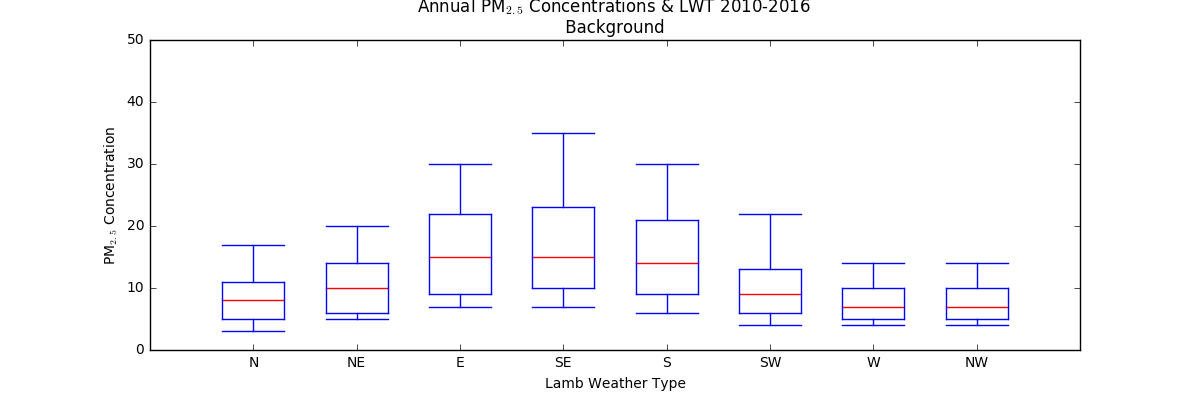
\includegraphics[height=6cm,left]{/nfs/see-fs-01_teaching/ee15amg/Paper_1/figures/boxplots/pm25_lwt_annual_data_check.png}
    \caption{Annual observations of PM$_{2.5}$ concentration from AURN sites between 2010-2016 under different wind directions (in $\mu$gm$^{3}$). Mean concentratiions are shown in red with the IQR and 10$^{th}$ and 90$^{th}$ percentiles in blue.}
    \label{fig:annual_boxplot}
\end{figure}

\begin{figure}[!ht]
  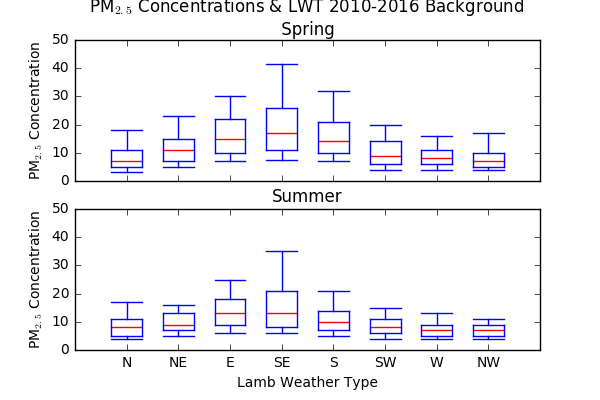
\includegraphics[height=6cm]{/nfs/see-fs-01_teaching/ee15amg/Paper_1/figures/boxplots/monthly_check_lwt_seasonal_spring_summer.png}
  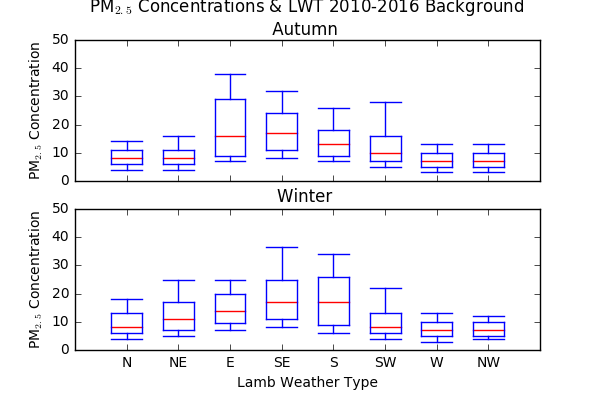
\includegraphics[height=6cm]{/nfs/see-fs-01_teaching/ee15amg/Paper_1/figures/boxplots/monthly_check_lwt_seasonal_autumn_winter.png}
  \caption{Seasonal observations of PM$_{2.5}$ concentration from AURN sites between 2010-2016 under different wind directions (in $\mu$gm$^{3}$). Mean concentratiions are shown in red with the IQR and 10$^{th}$ and 90$^{th}$ percentiles in blue.}
  \label{fig:seasonal_boxplot}
\end{figure}

- Annual plots
\begin{enumerate}
\item Annual SE, S, E = highest PM2.5 mean and 75th/95th percentiles
\item Annual W, NW, N = lowest PM2.5 mean and 75th/95th percentiles
\item Annual 10th and 25th percentile also much higher in SE, S, E flow
\end{enumerate}

- Seasonal Plots
\begin{enumerate}
\item S/S - SE, S, E also highest again, W,NW lowest 
\item Spring SE (>40 ugm3) = highest concentrations observed, 90th and 75th percentiles of NW,W and N also elevated during spring compared to other months
\item Autumn - E = higher concs than other months (almost 40ugm3) and SW also higher than southerly.
\item Winter - SE and S highest pollution, both give similar values (35 ugm3) 
\end{enumerate}


Annually the highest mean, 75$^{th}$ and 90$^{th}$ percentile PM$_{2.5}$ concentrations occur under easterly (E), south-easterly (SE) and southerly (S) lamb weather types (LWTs) (Fig. \ref{fig:annual_boxplot}). Averaged over all sites this gives a 90$^{th}$ percentile concentration of 35$\mu$gm$^{-3}$, ranging from 10 - 50 $\mu$gm$^{-3}$ (Fig. \ref{fig:annual_90th_values}).

\subsection*{Concentration Maps}

\begin{figure}
	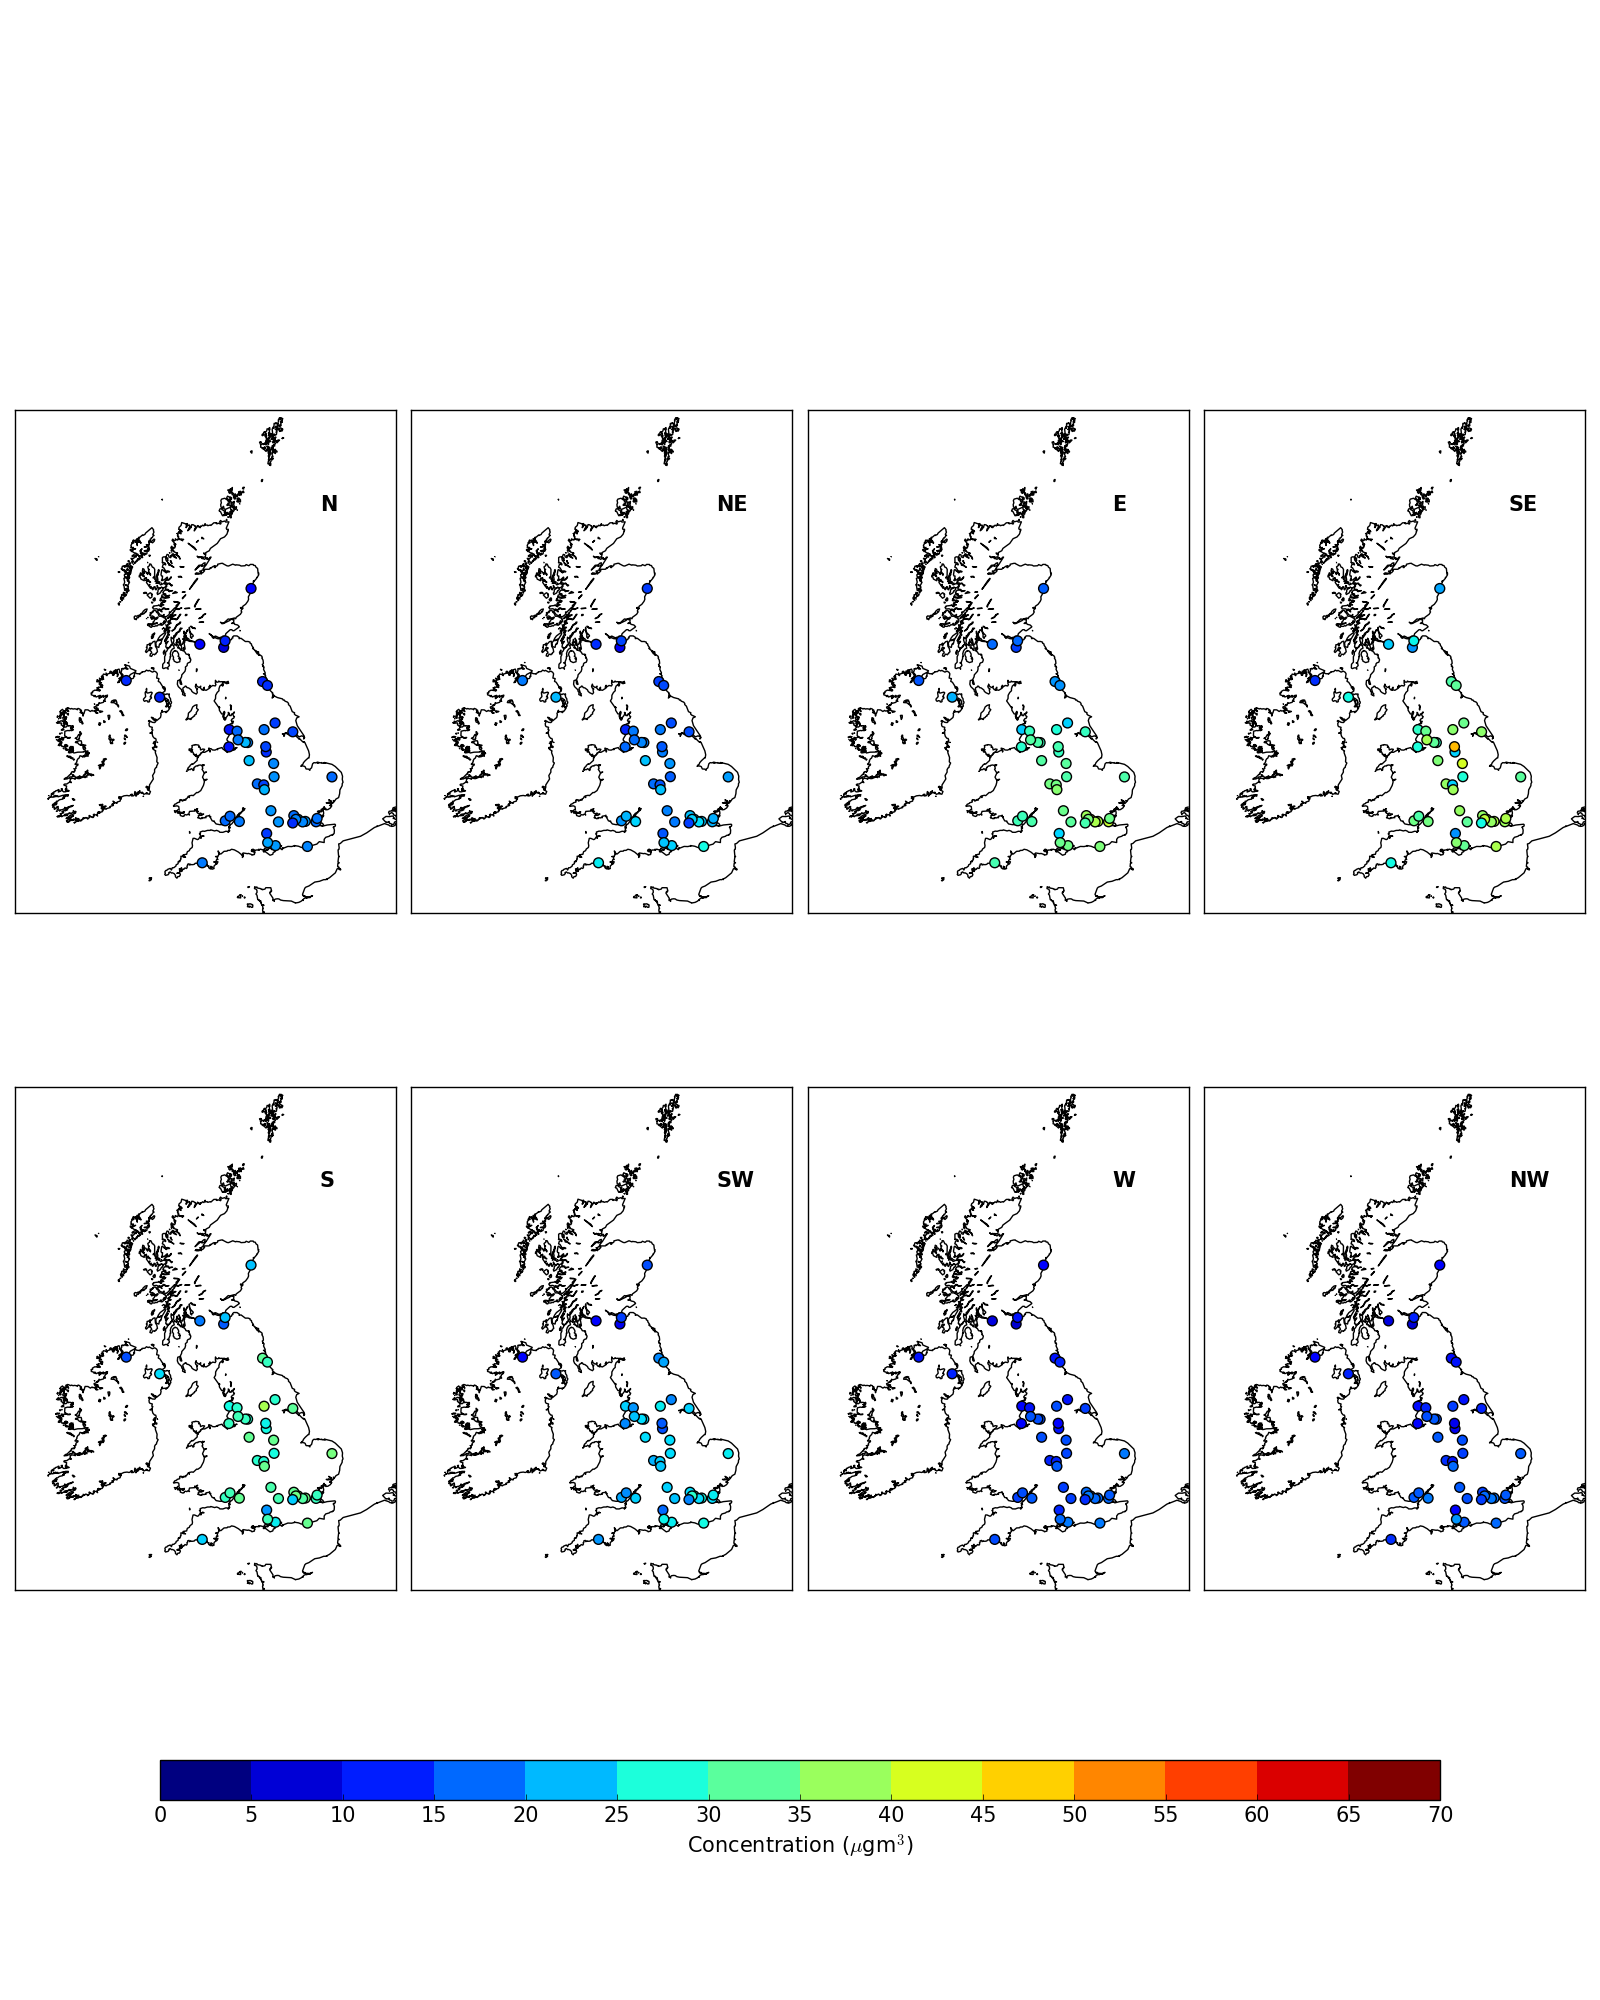
\includegraphics[height=22cm]{/nfs/see-fs-01_teaching/ee15amg/Paper_1/figures/pm25_conc_maps/Annual_90th_percentile_lwt_values.png}
	\caption{Annual 90th Values}
	\label{fig:annual_90th_values}
\end{figure}

\begin{figure}
	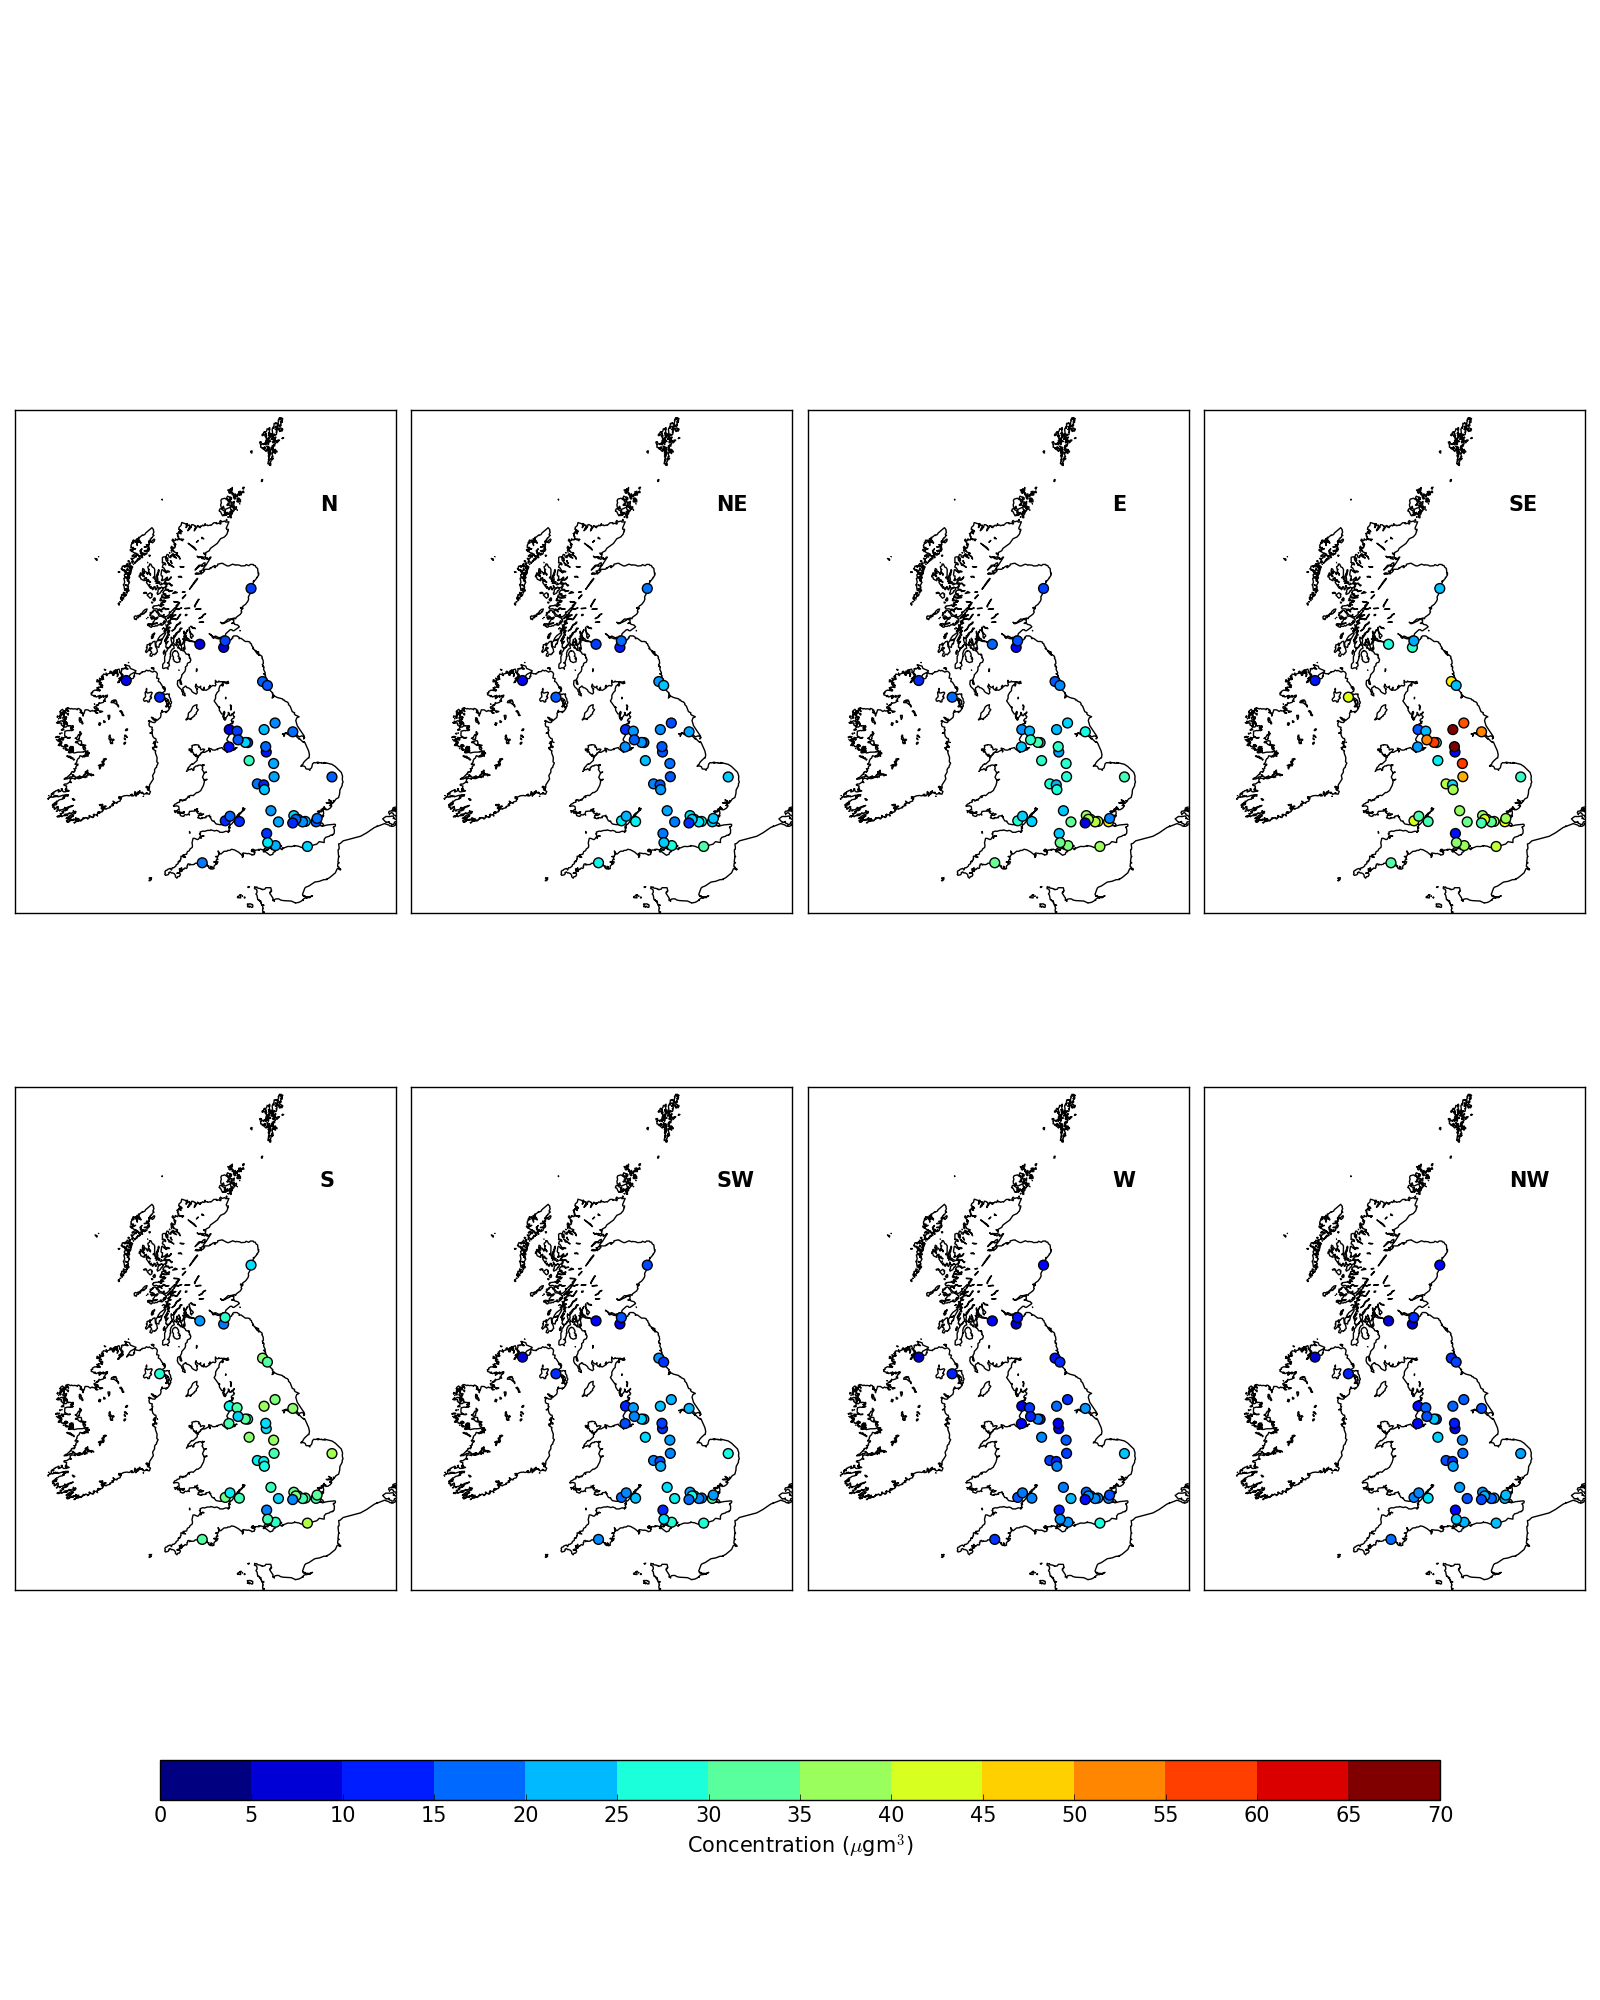
\includegraphics[height=22cm]{/nfs/see-fs-01_teaching/ee15amg/Paper_1/figures/pm25_conc_maps/Spring_90th_percentile_values.png}
	\caption{Spring 90th Values}
\end{figure}

\begin{figure}
	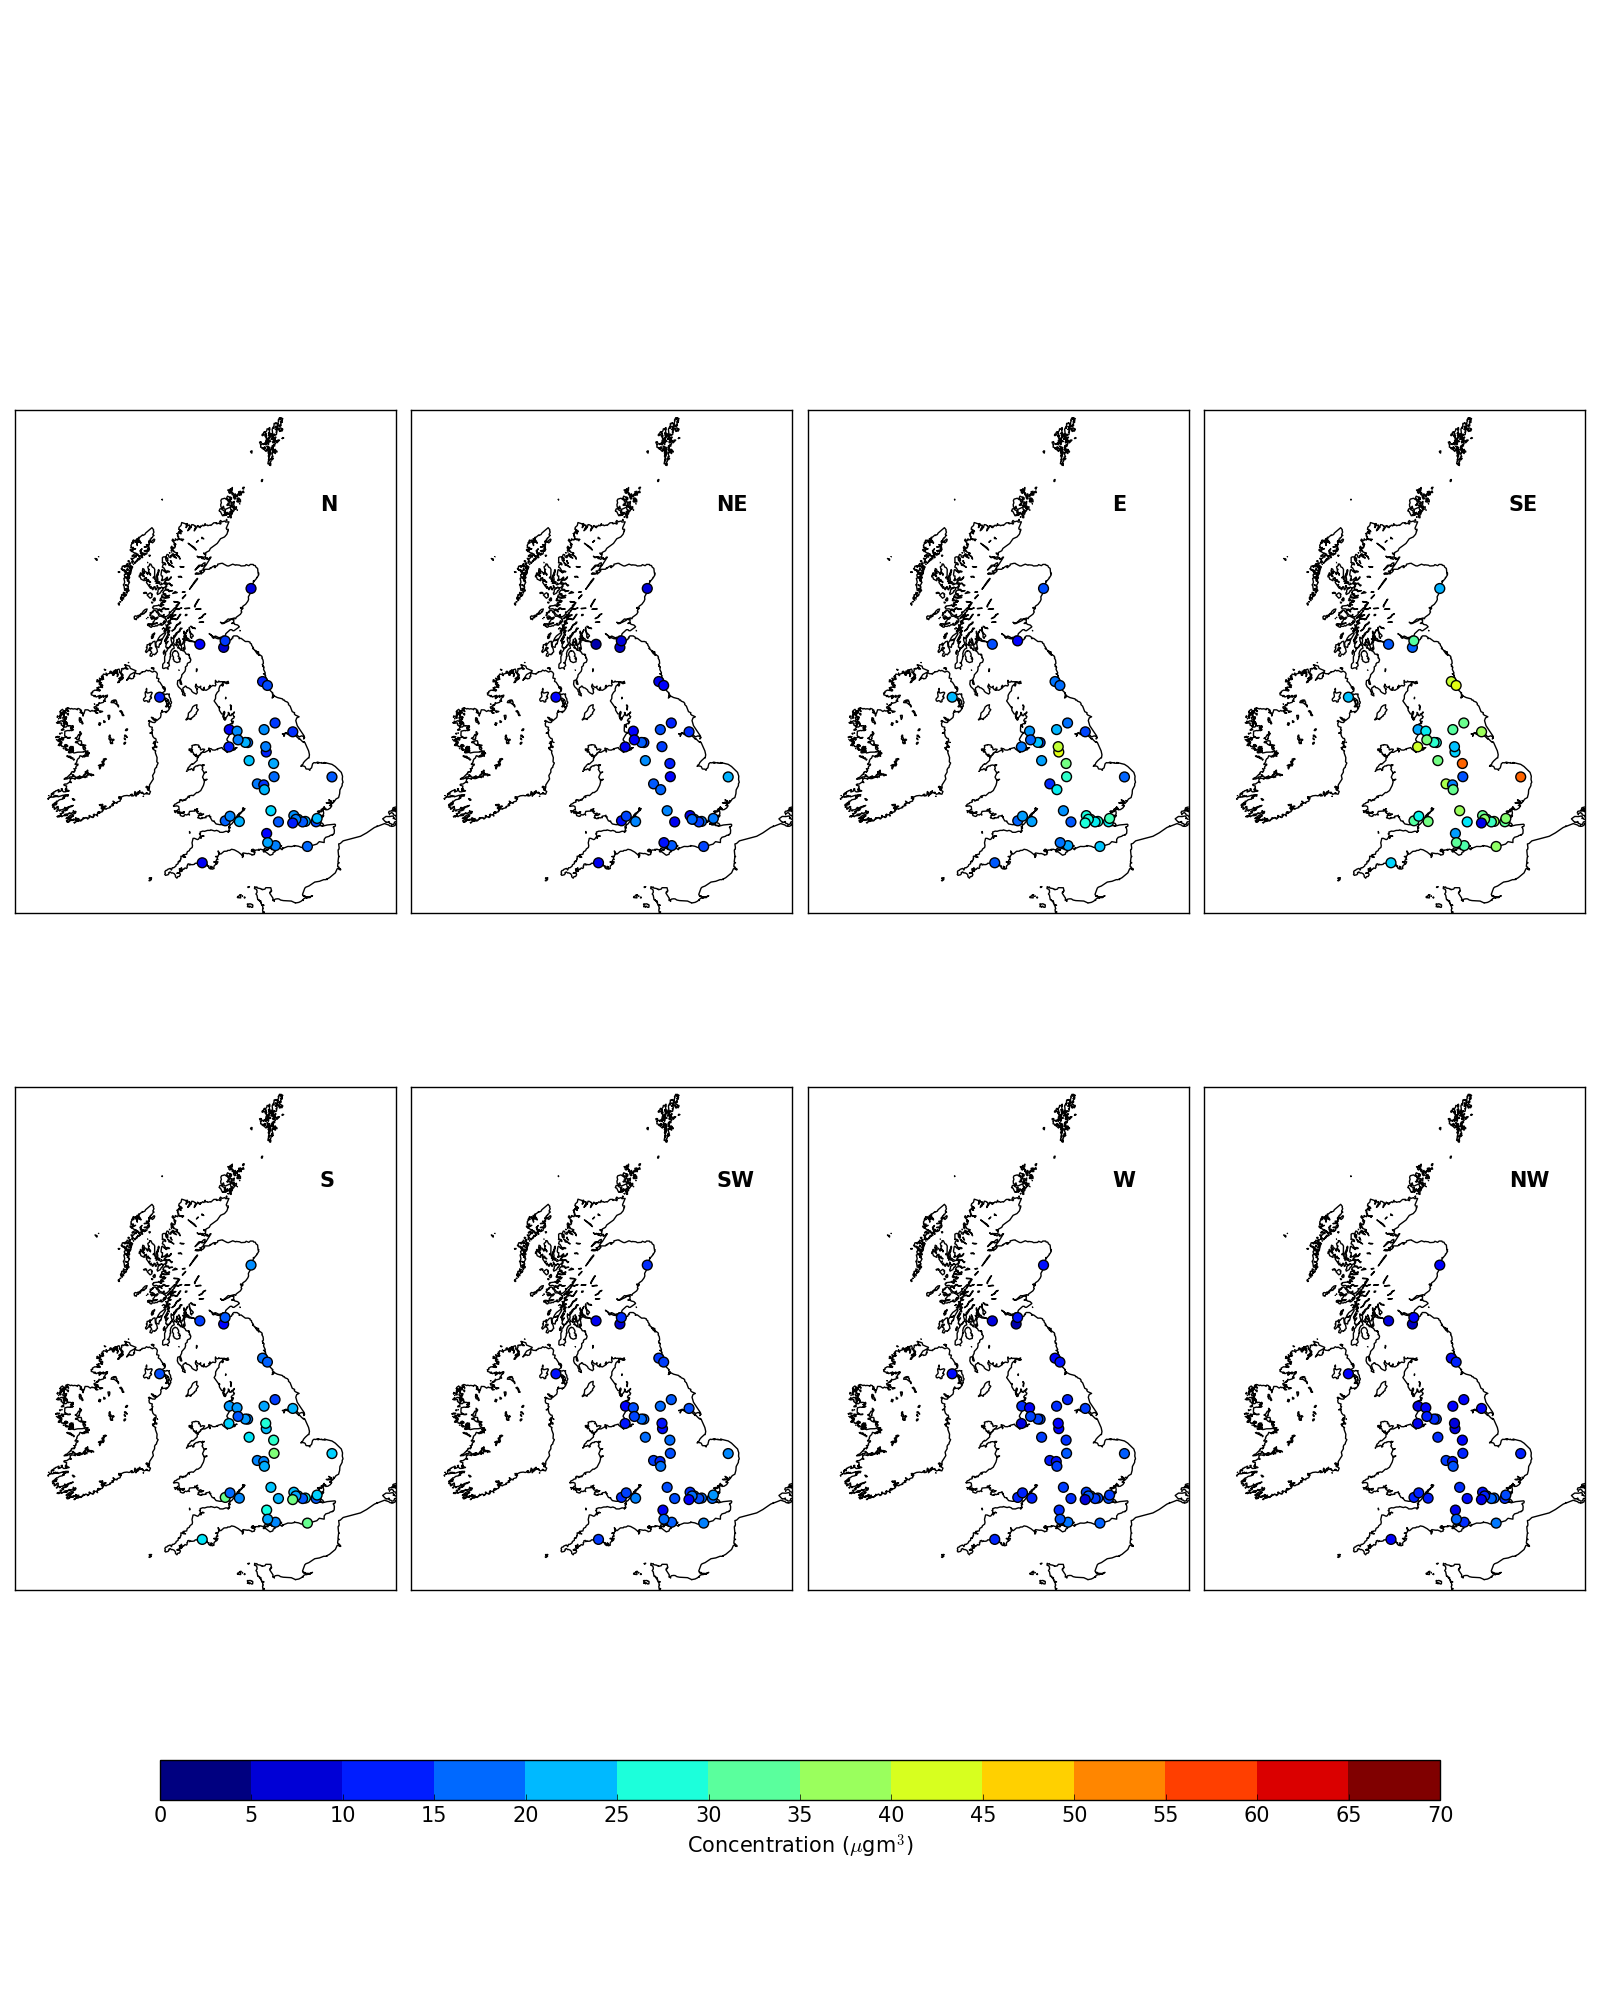
\includegraphics[height=22cm]{/nfs/see-fs-01_teaching/ee15amg/Paper_1/figures/pm25_conc_maps/Summer_90th_percentile_values.png}
	\caption{Summer 90th Values}
\end{figure}

\begin{figure}
	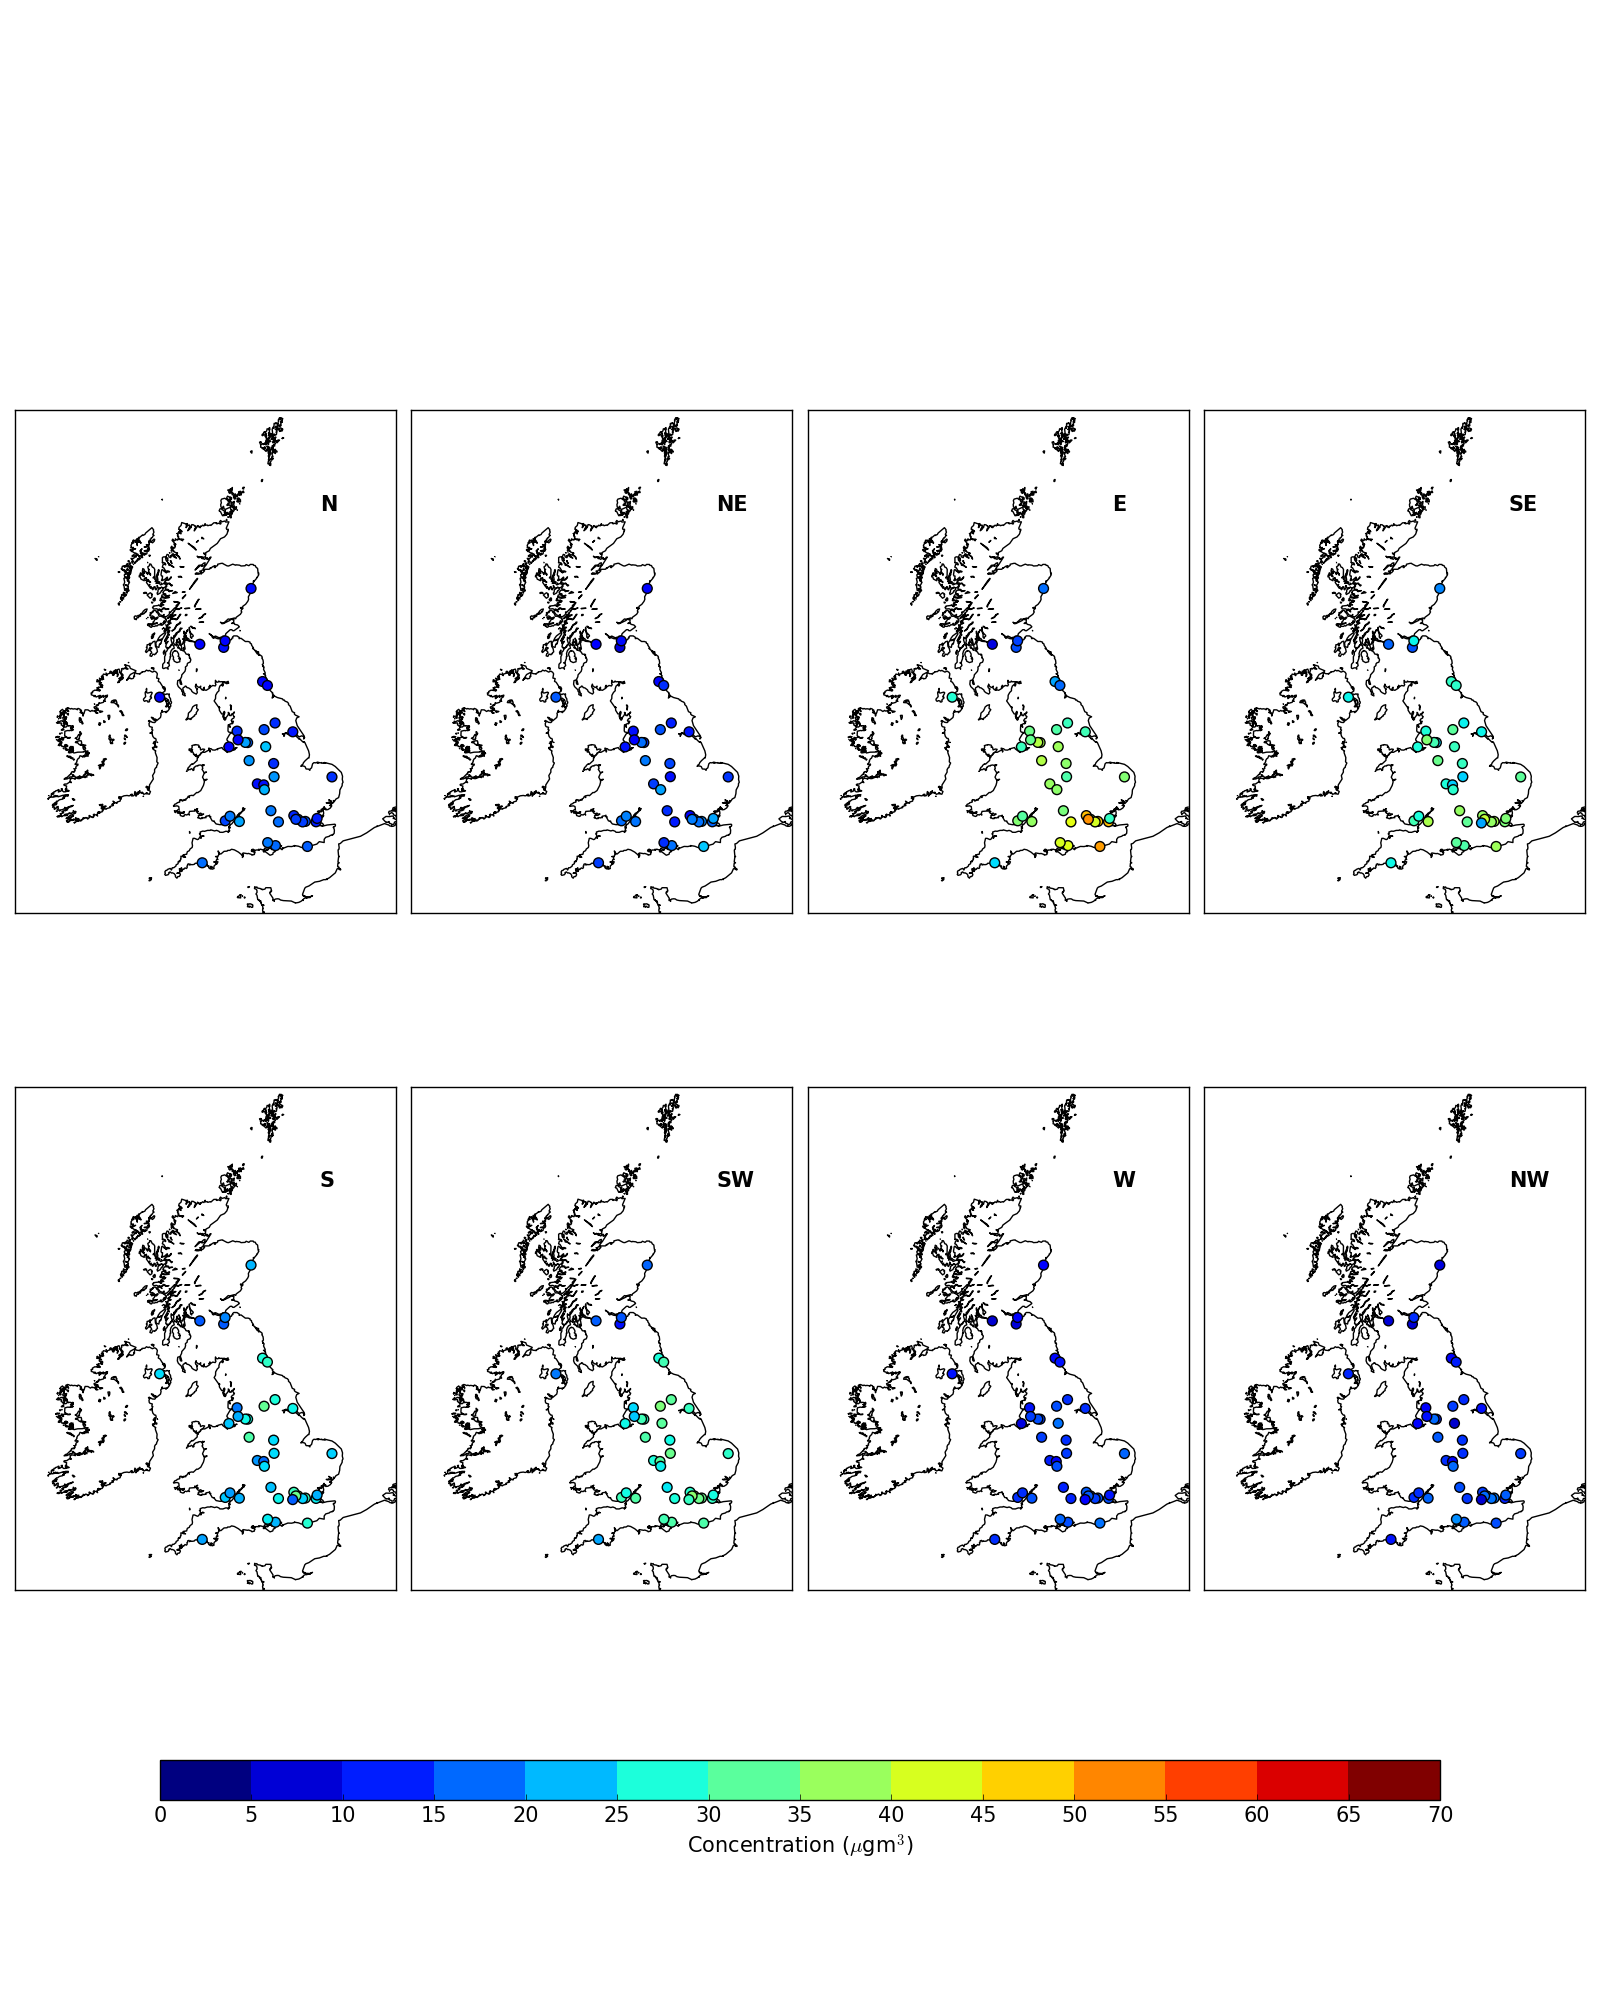
\includegraphics[height=22cm]{/nfs/see-fs-01_teaching/ee15amg/Paper_1/figures/pm25_conc_maps/Autumn_90th_percentile_values.png}
	\caption{Autumn 90th Values}
\end{figure}

\begin{figure}
	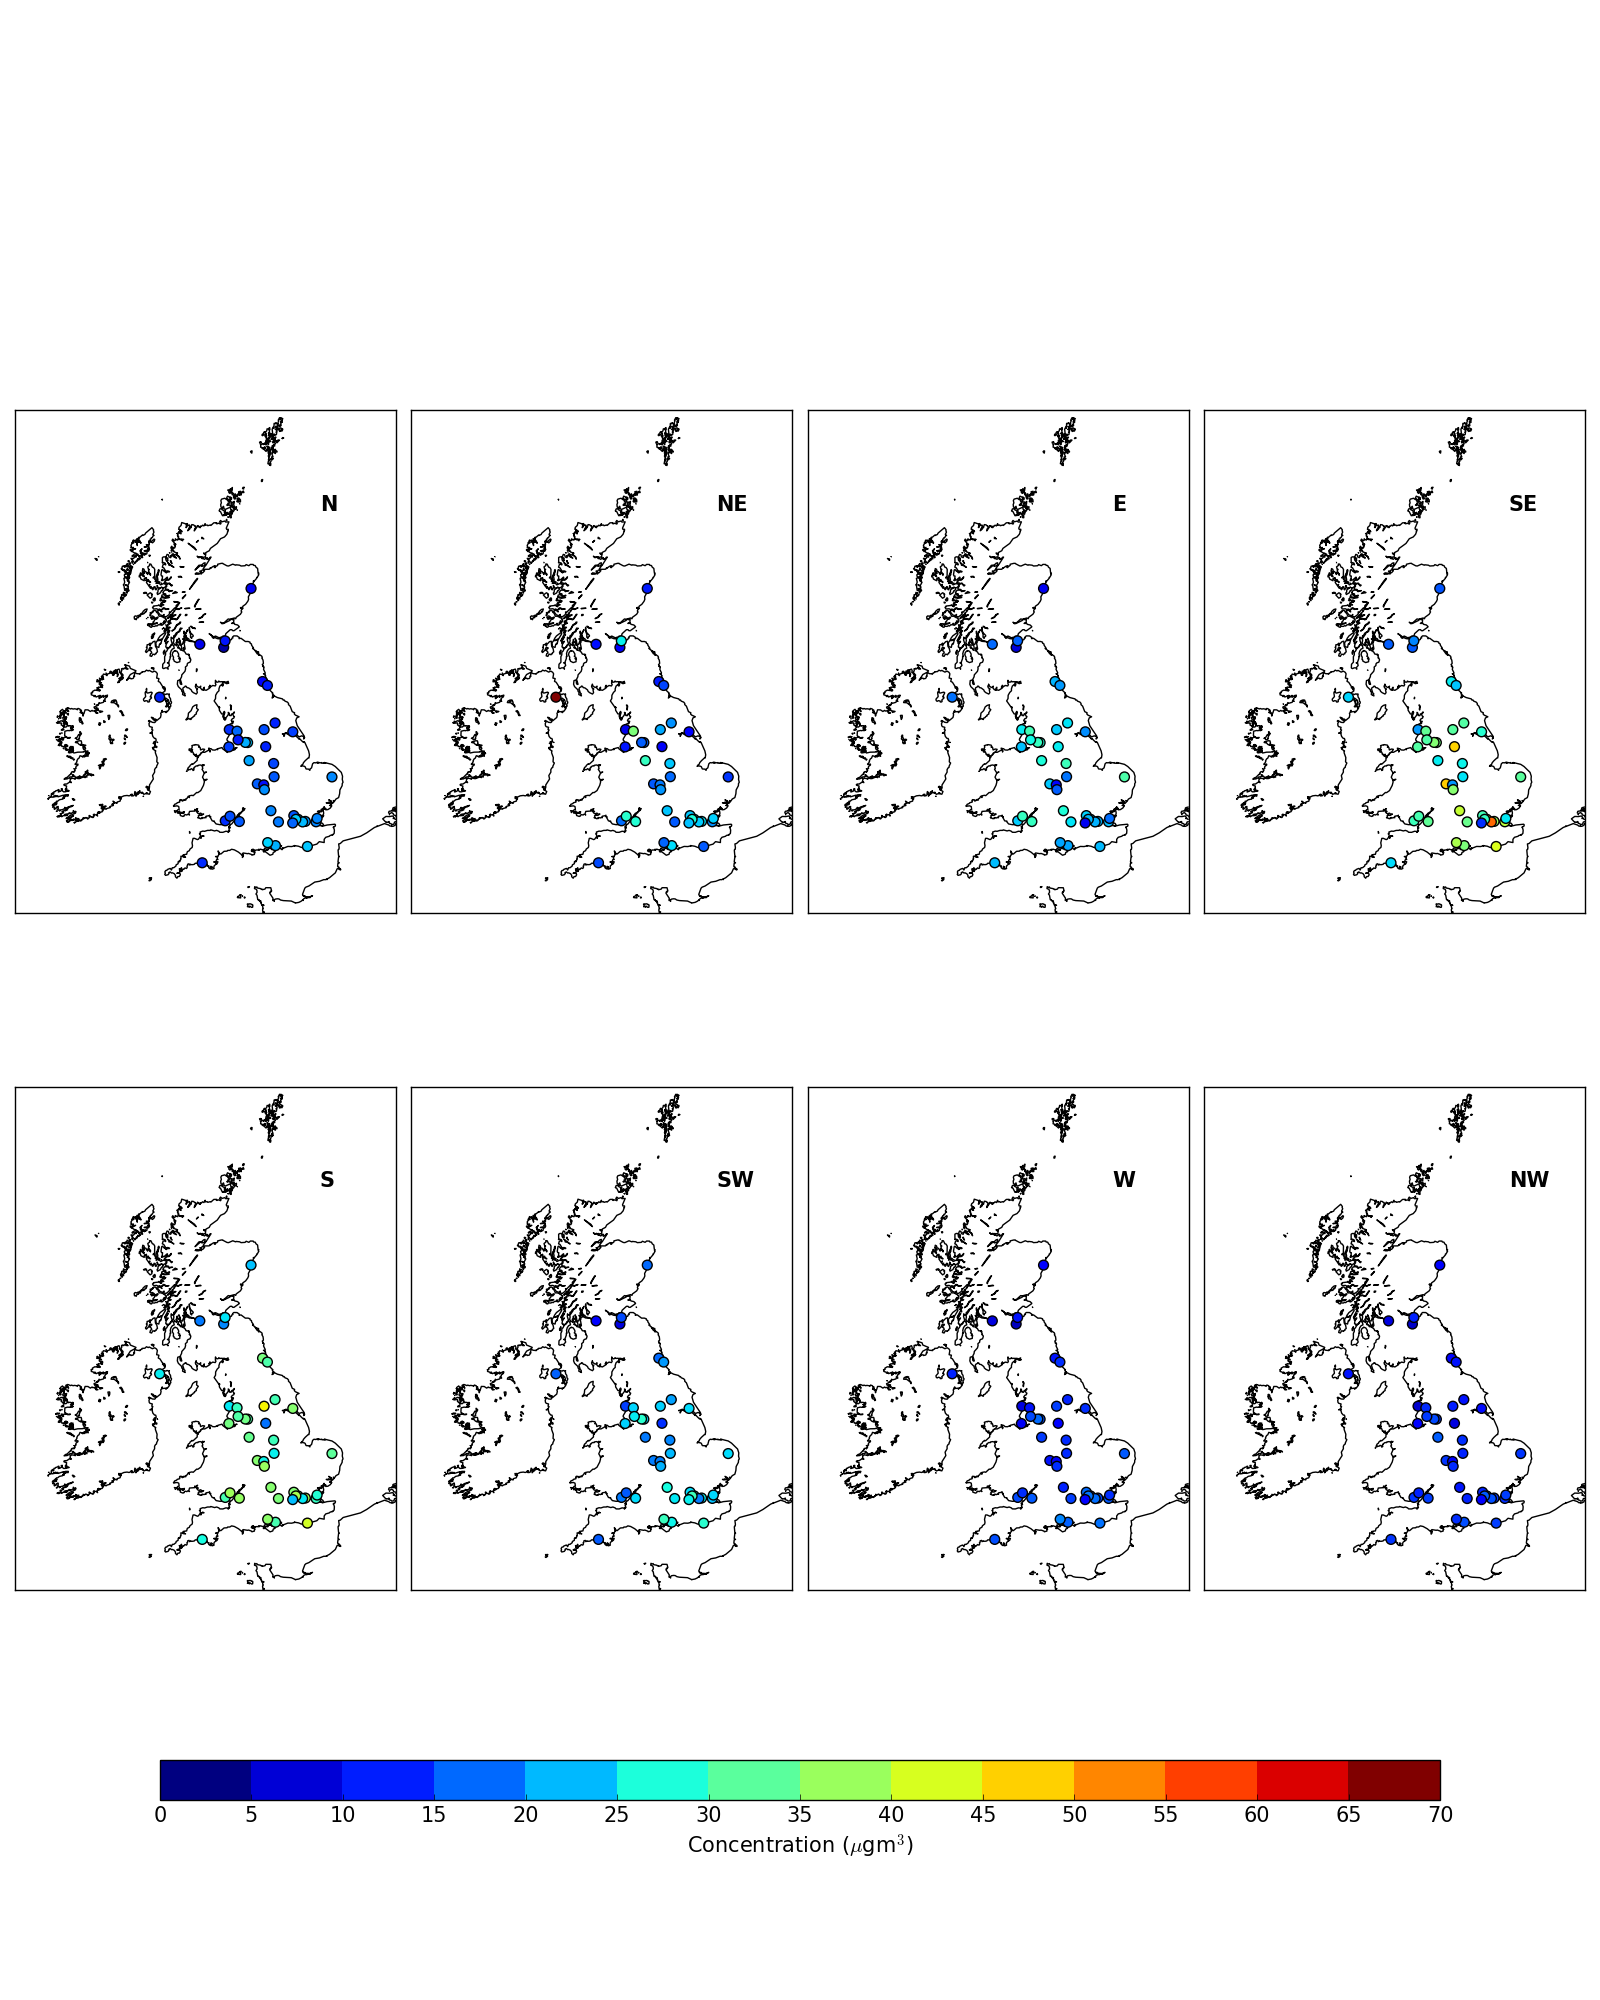
\includegraphics[height=22cm]{/nfs/see-fs-01_teaching/ee15amg/Paper_1/figures/pm25_conc_maps/Winter_90th_percentile_values.png}
	\caption{Winter 90th Values}
\end{figure}




\subsection*{Anomaly Plots}


\begin{figure}
	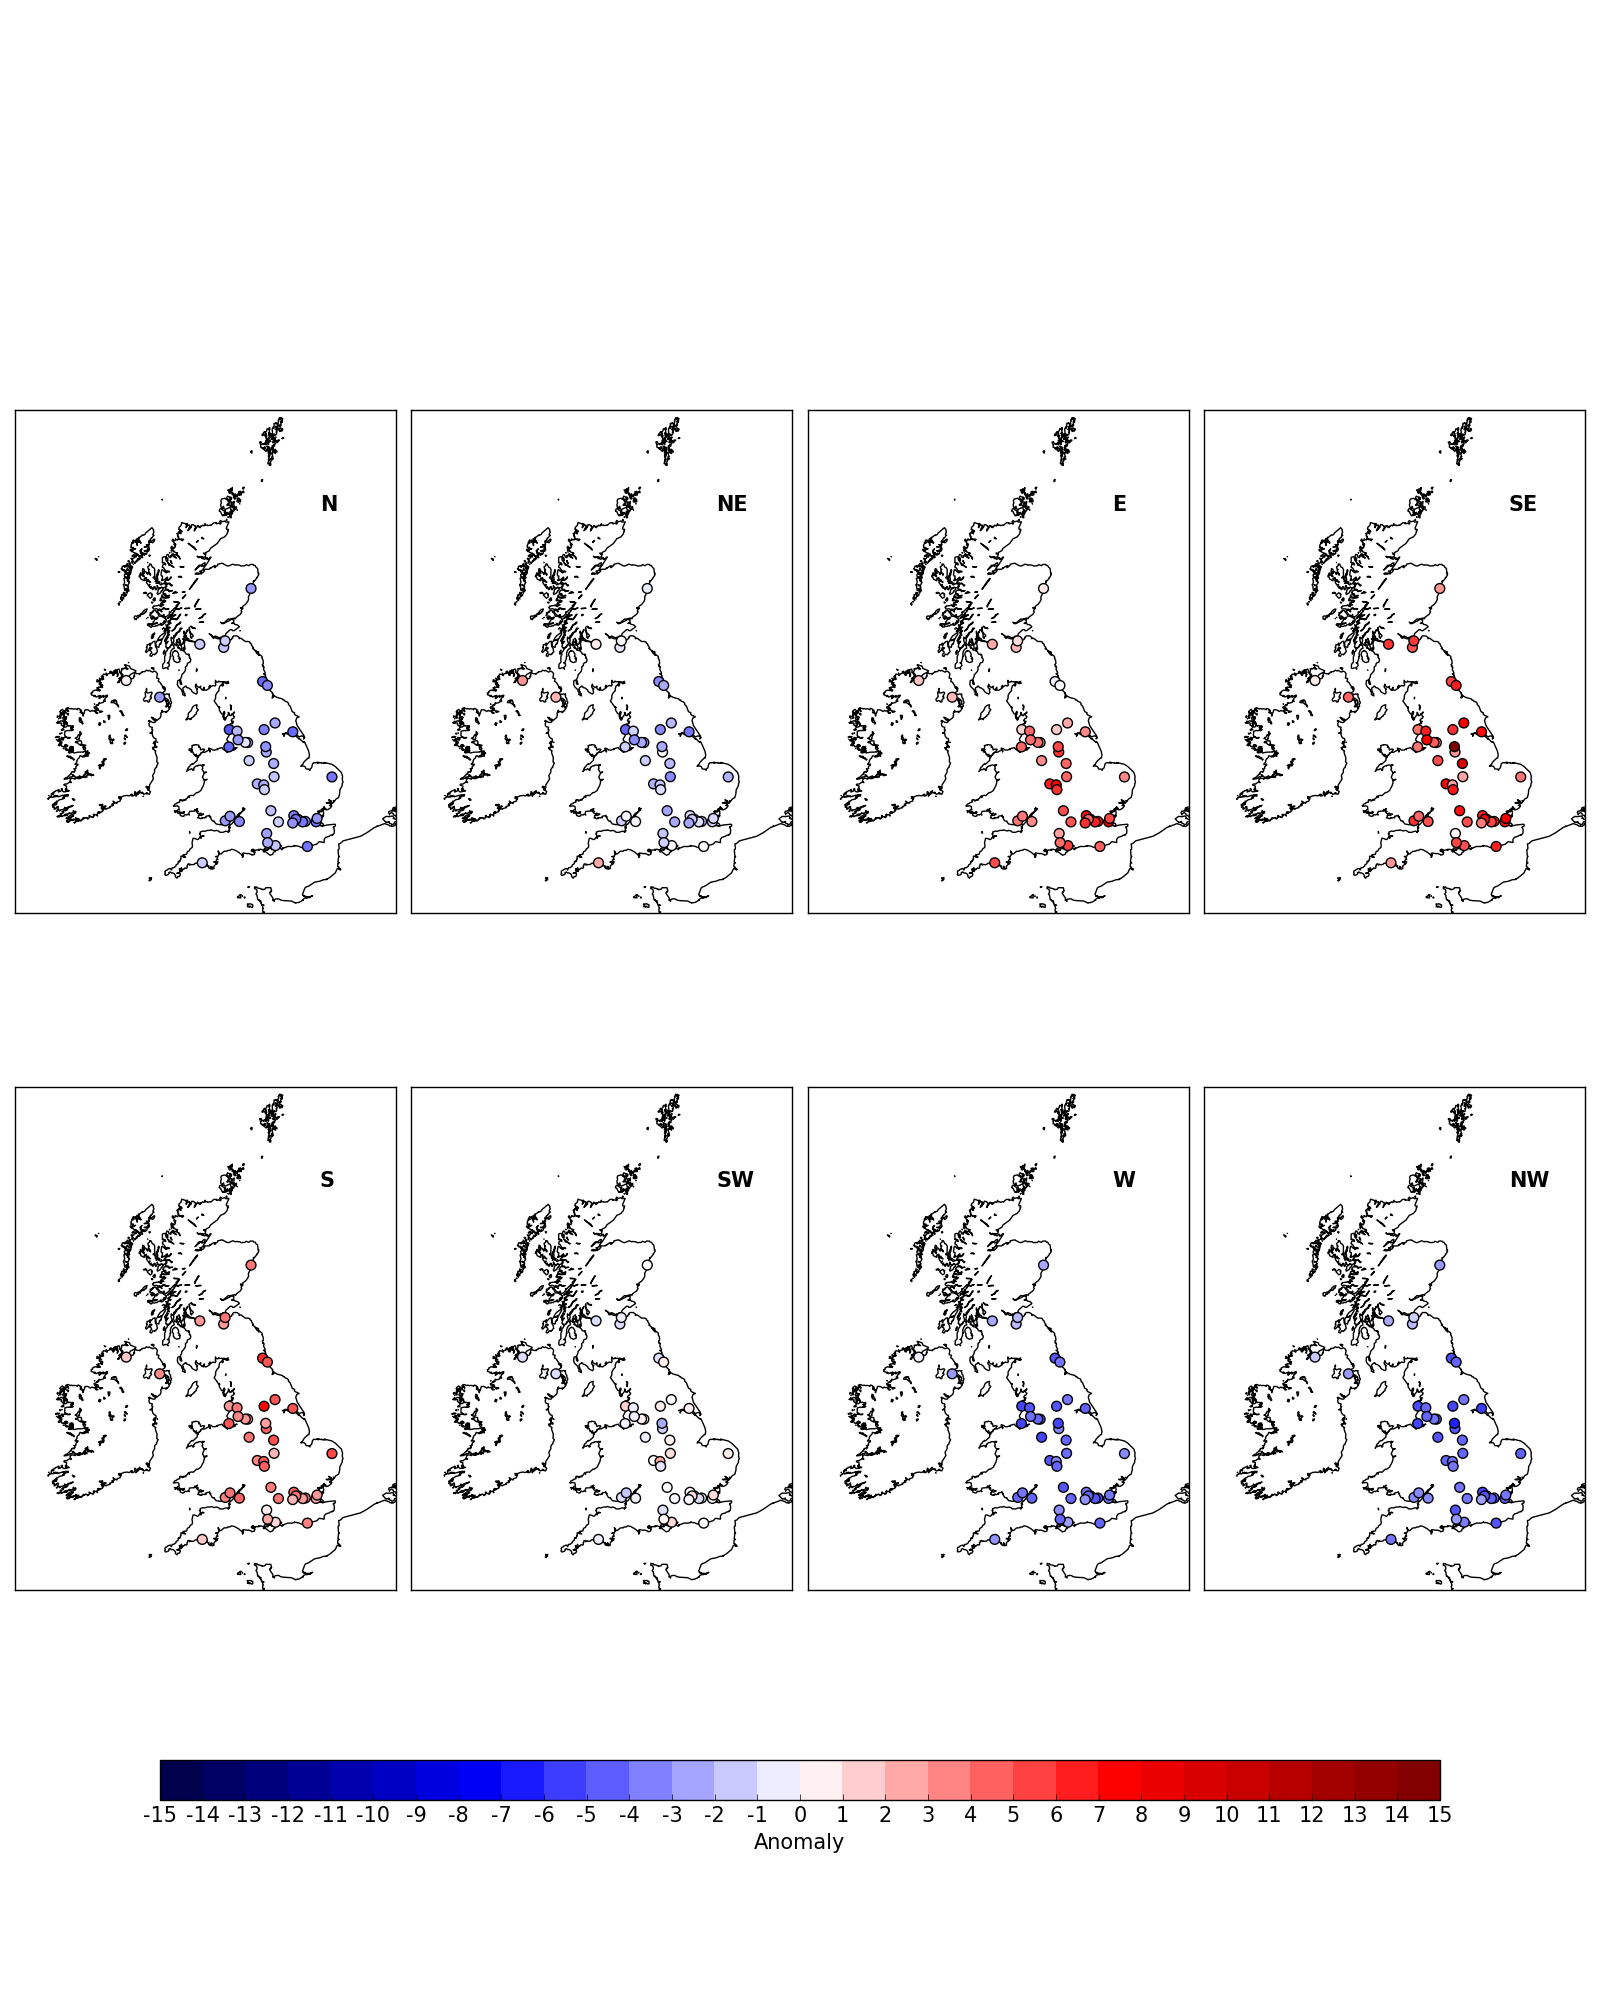
\includegraphics[height=22cm]{/nfs/see-fs-01_teaching/ee15amg/Paper_1/figures/anomalies/Annual_90th_percentile_lwt_anomalies.png}
	\caption{Annual 90th Anomaly}
\end{figure}


\begin{figure}
	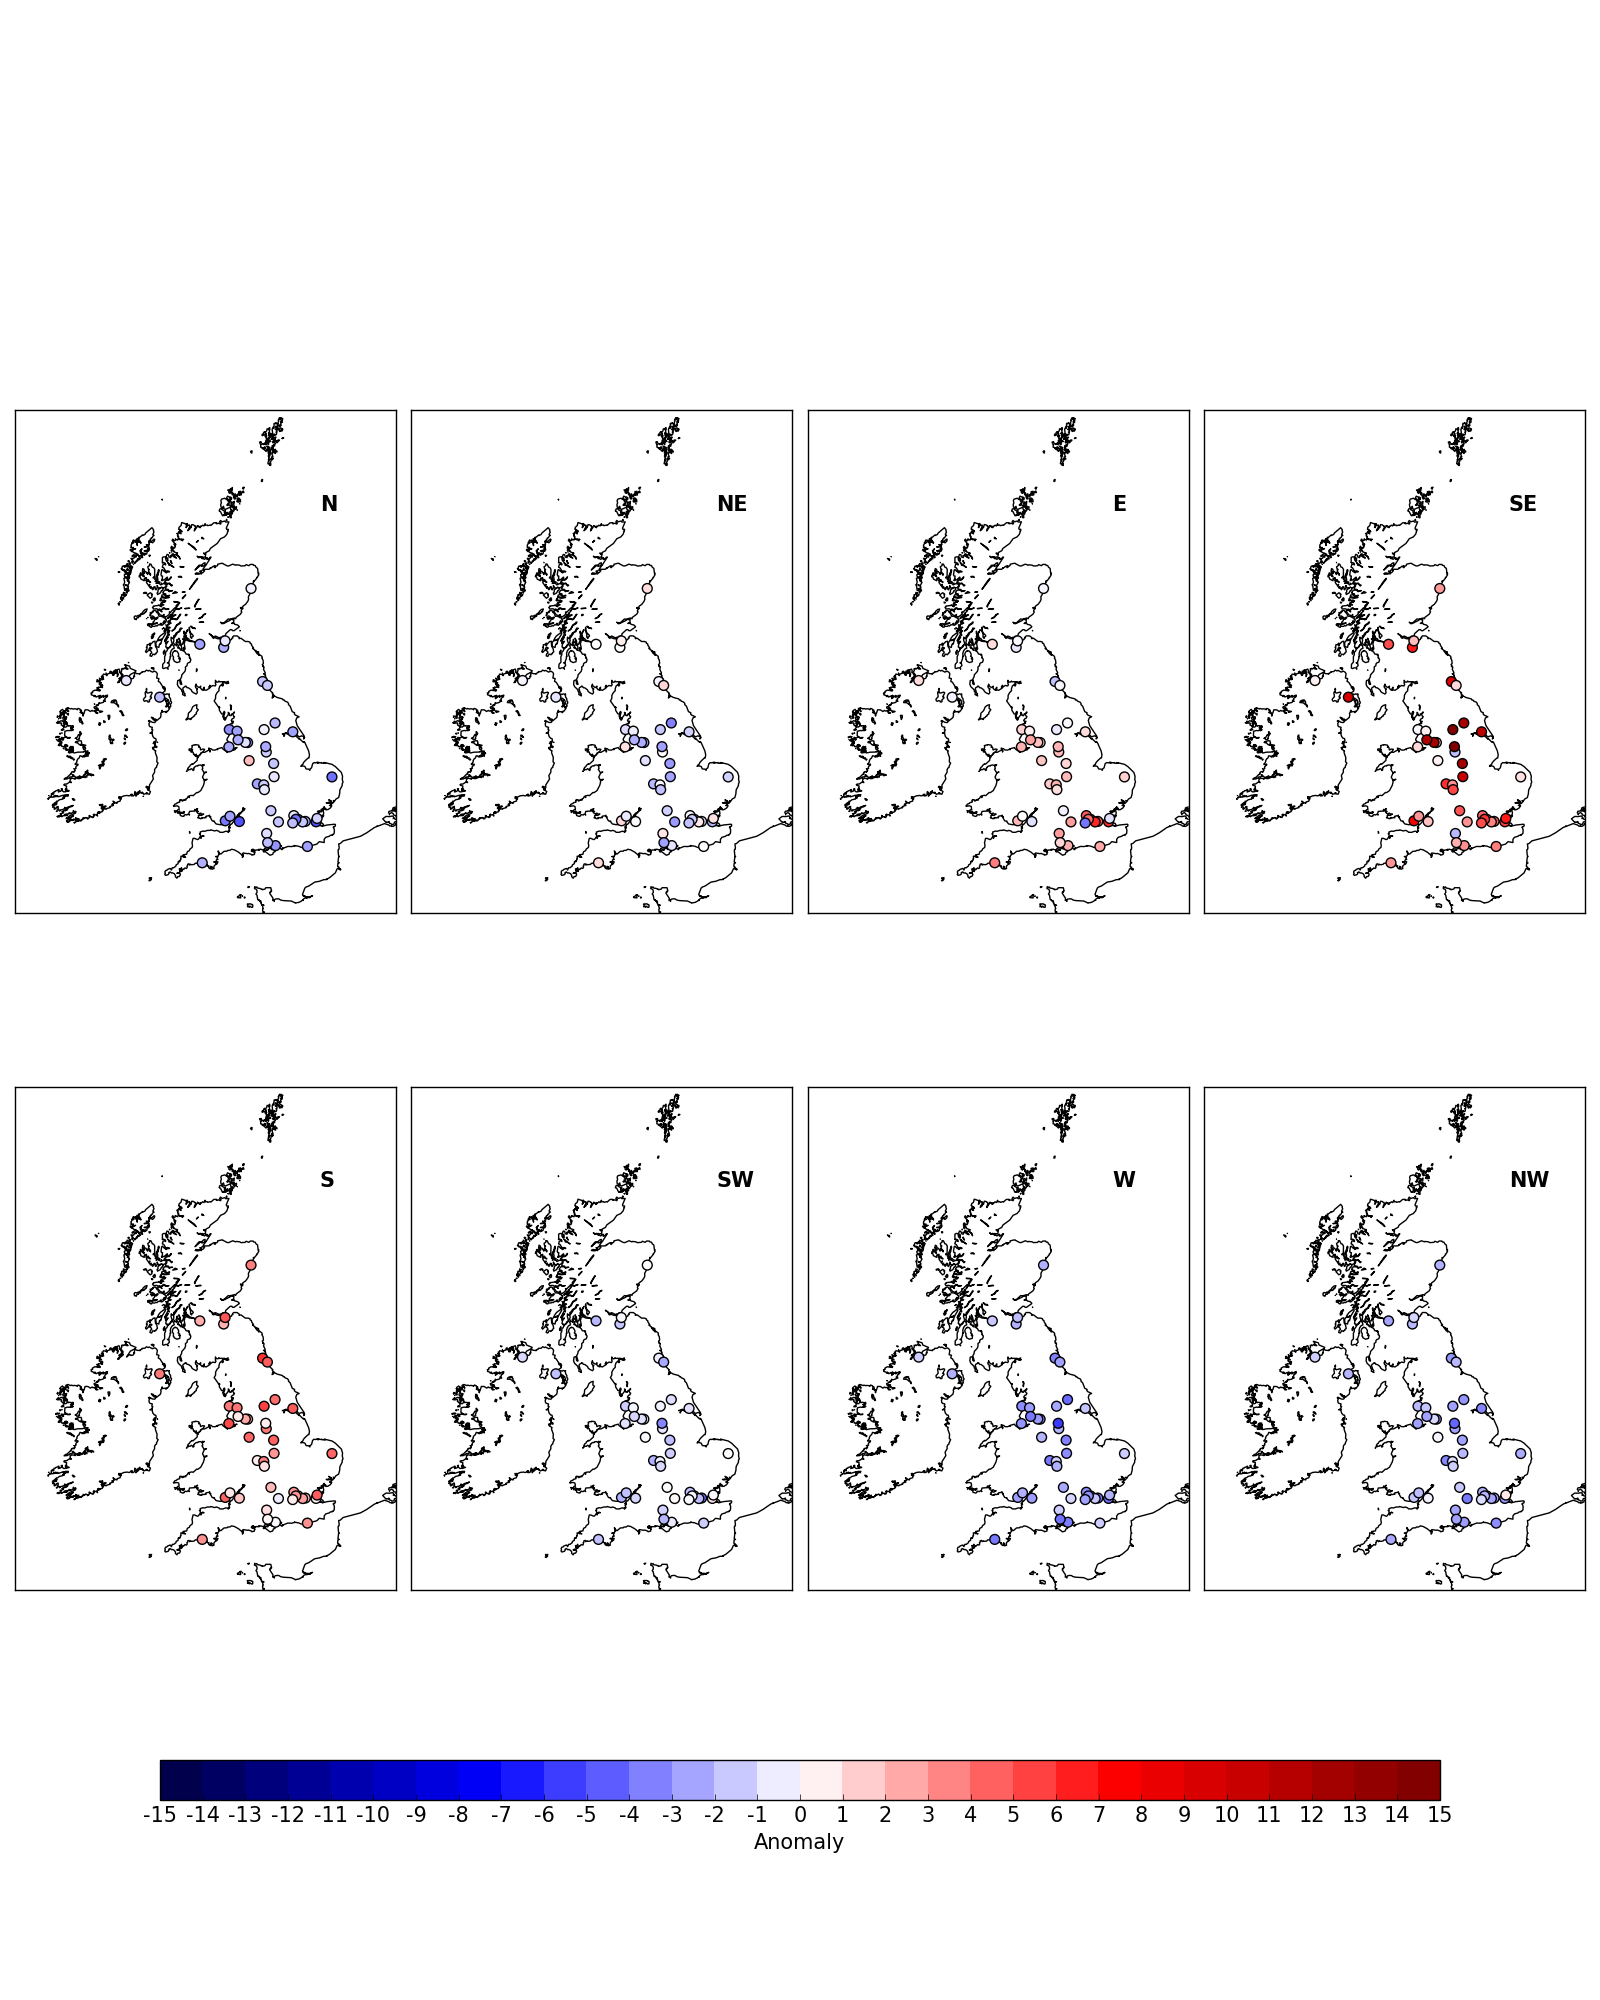
\includegraphics[height=22cm]{/nfs/see-fs-01_teaching/ee15amg/Paper_1/figures/anomalies/Spring_90th_percentile_anomalies.png}
	\caption{Spring 90th Anomaly}
\end{figure}


\begin{figure}
	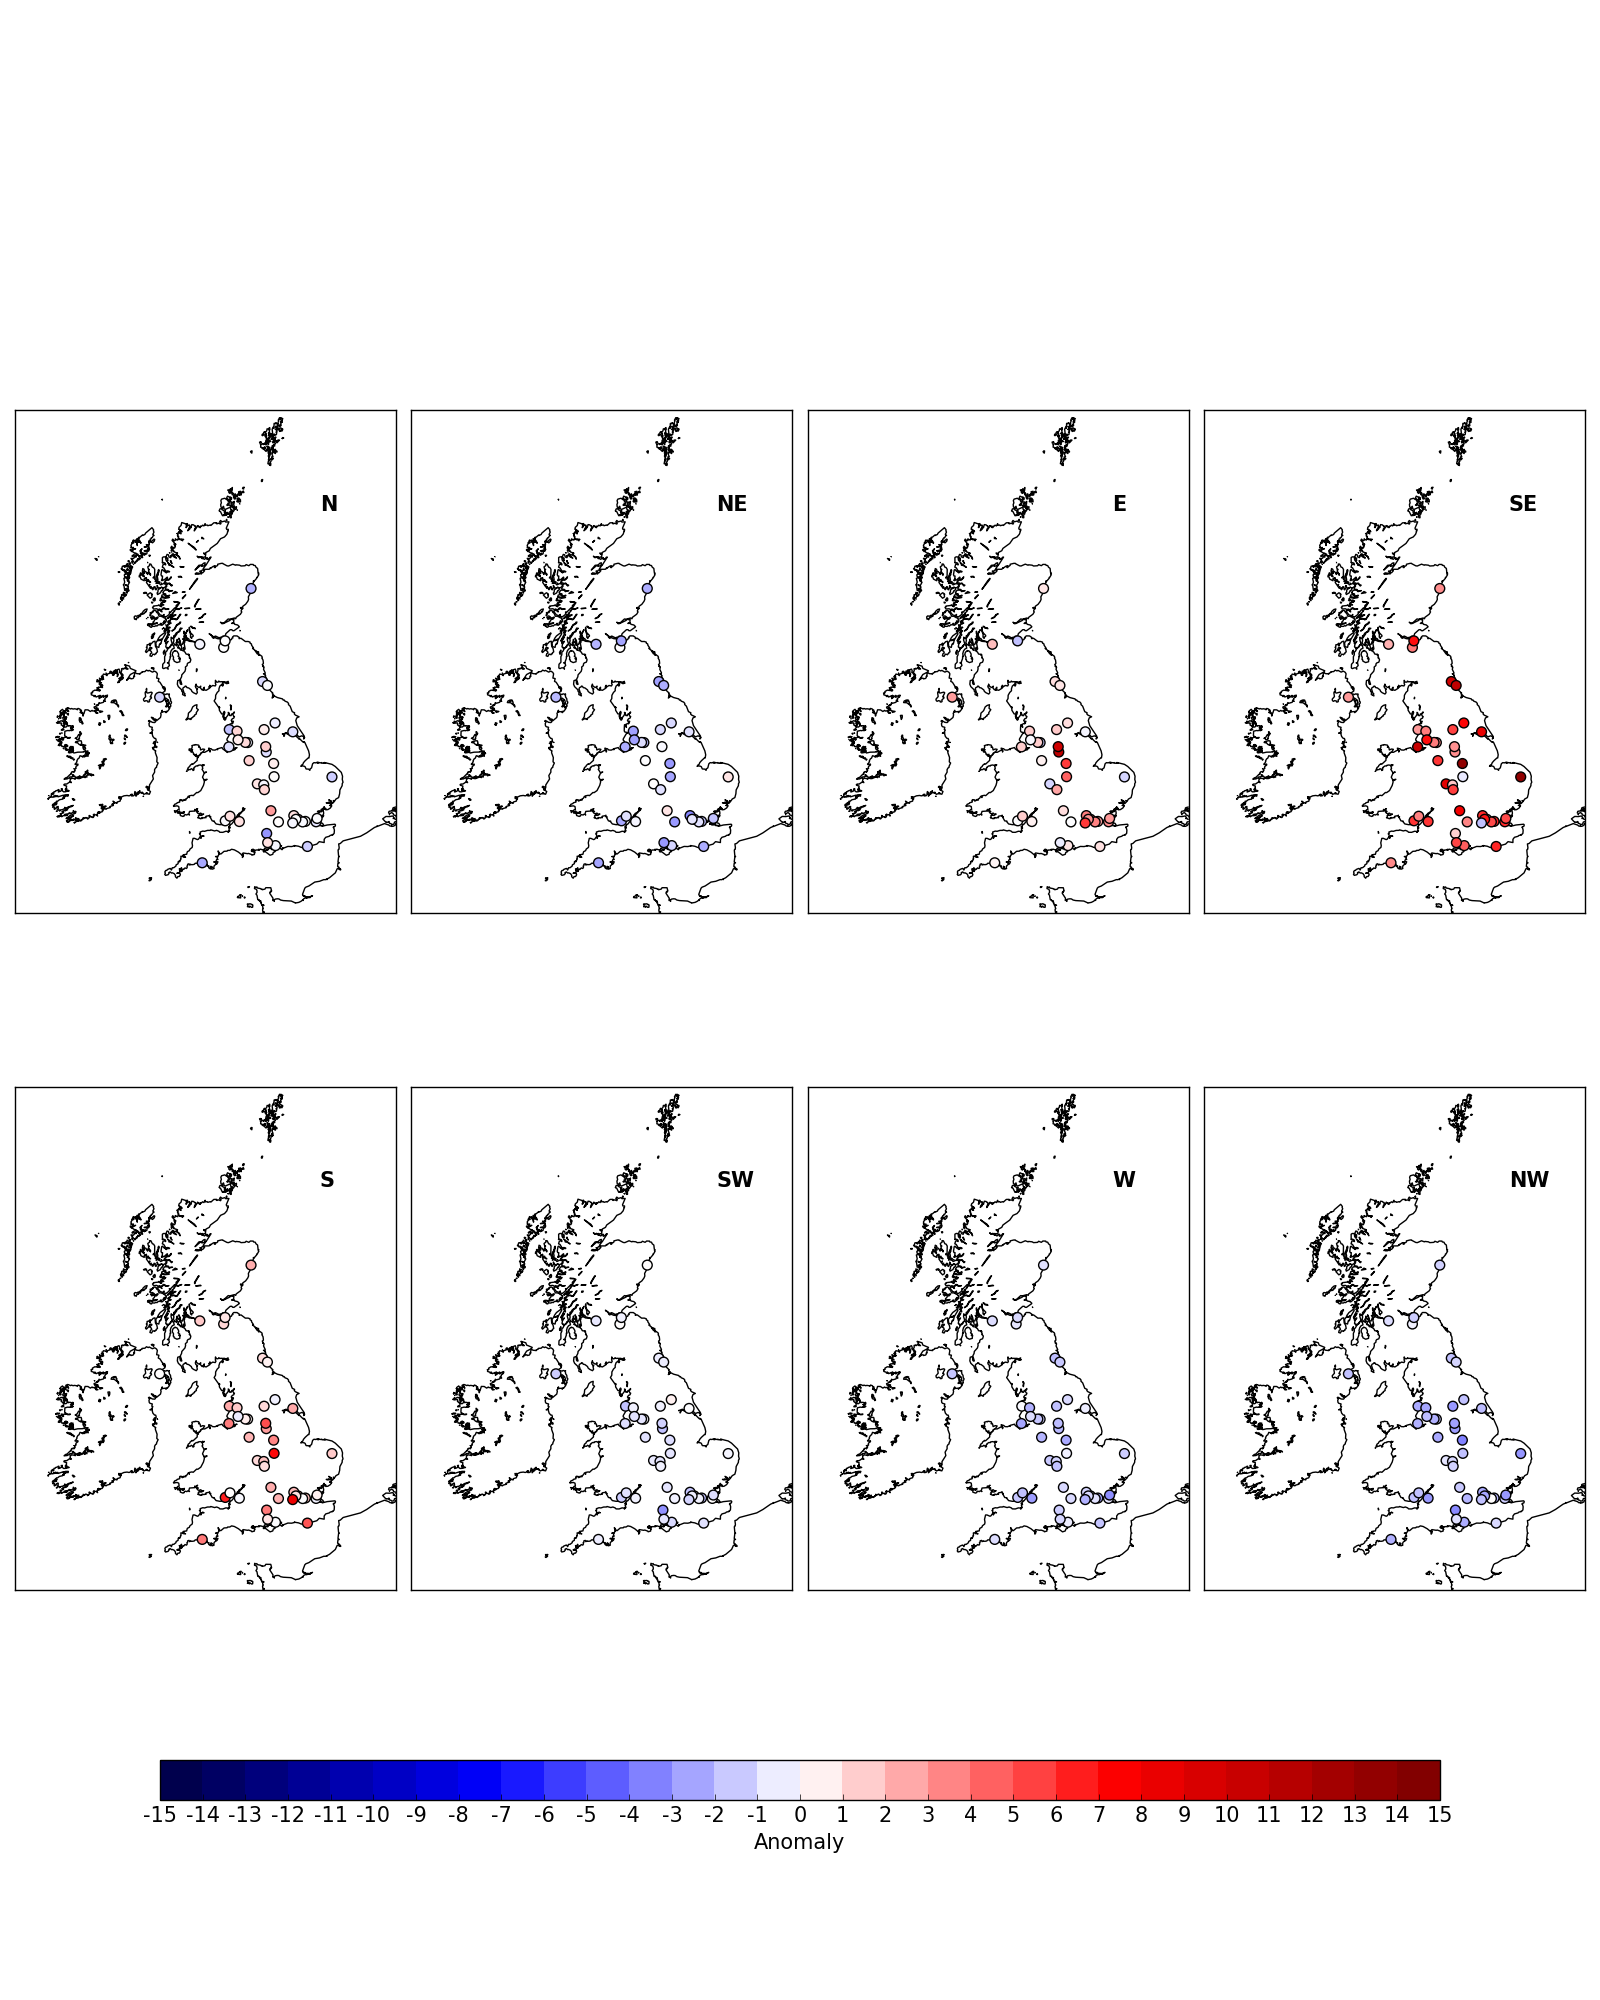
\includegraphics[height=22cm]{/nfs/see-fs-01_teaching/ee15amg/Paper_1/figures/anomalies/Summer_90th_percentile_anomalies.png}
	\caption{Summer 90th Anomaly}
\end{figure}

\begin{figure}
	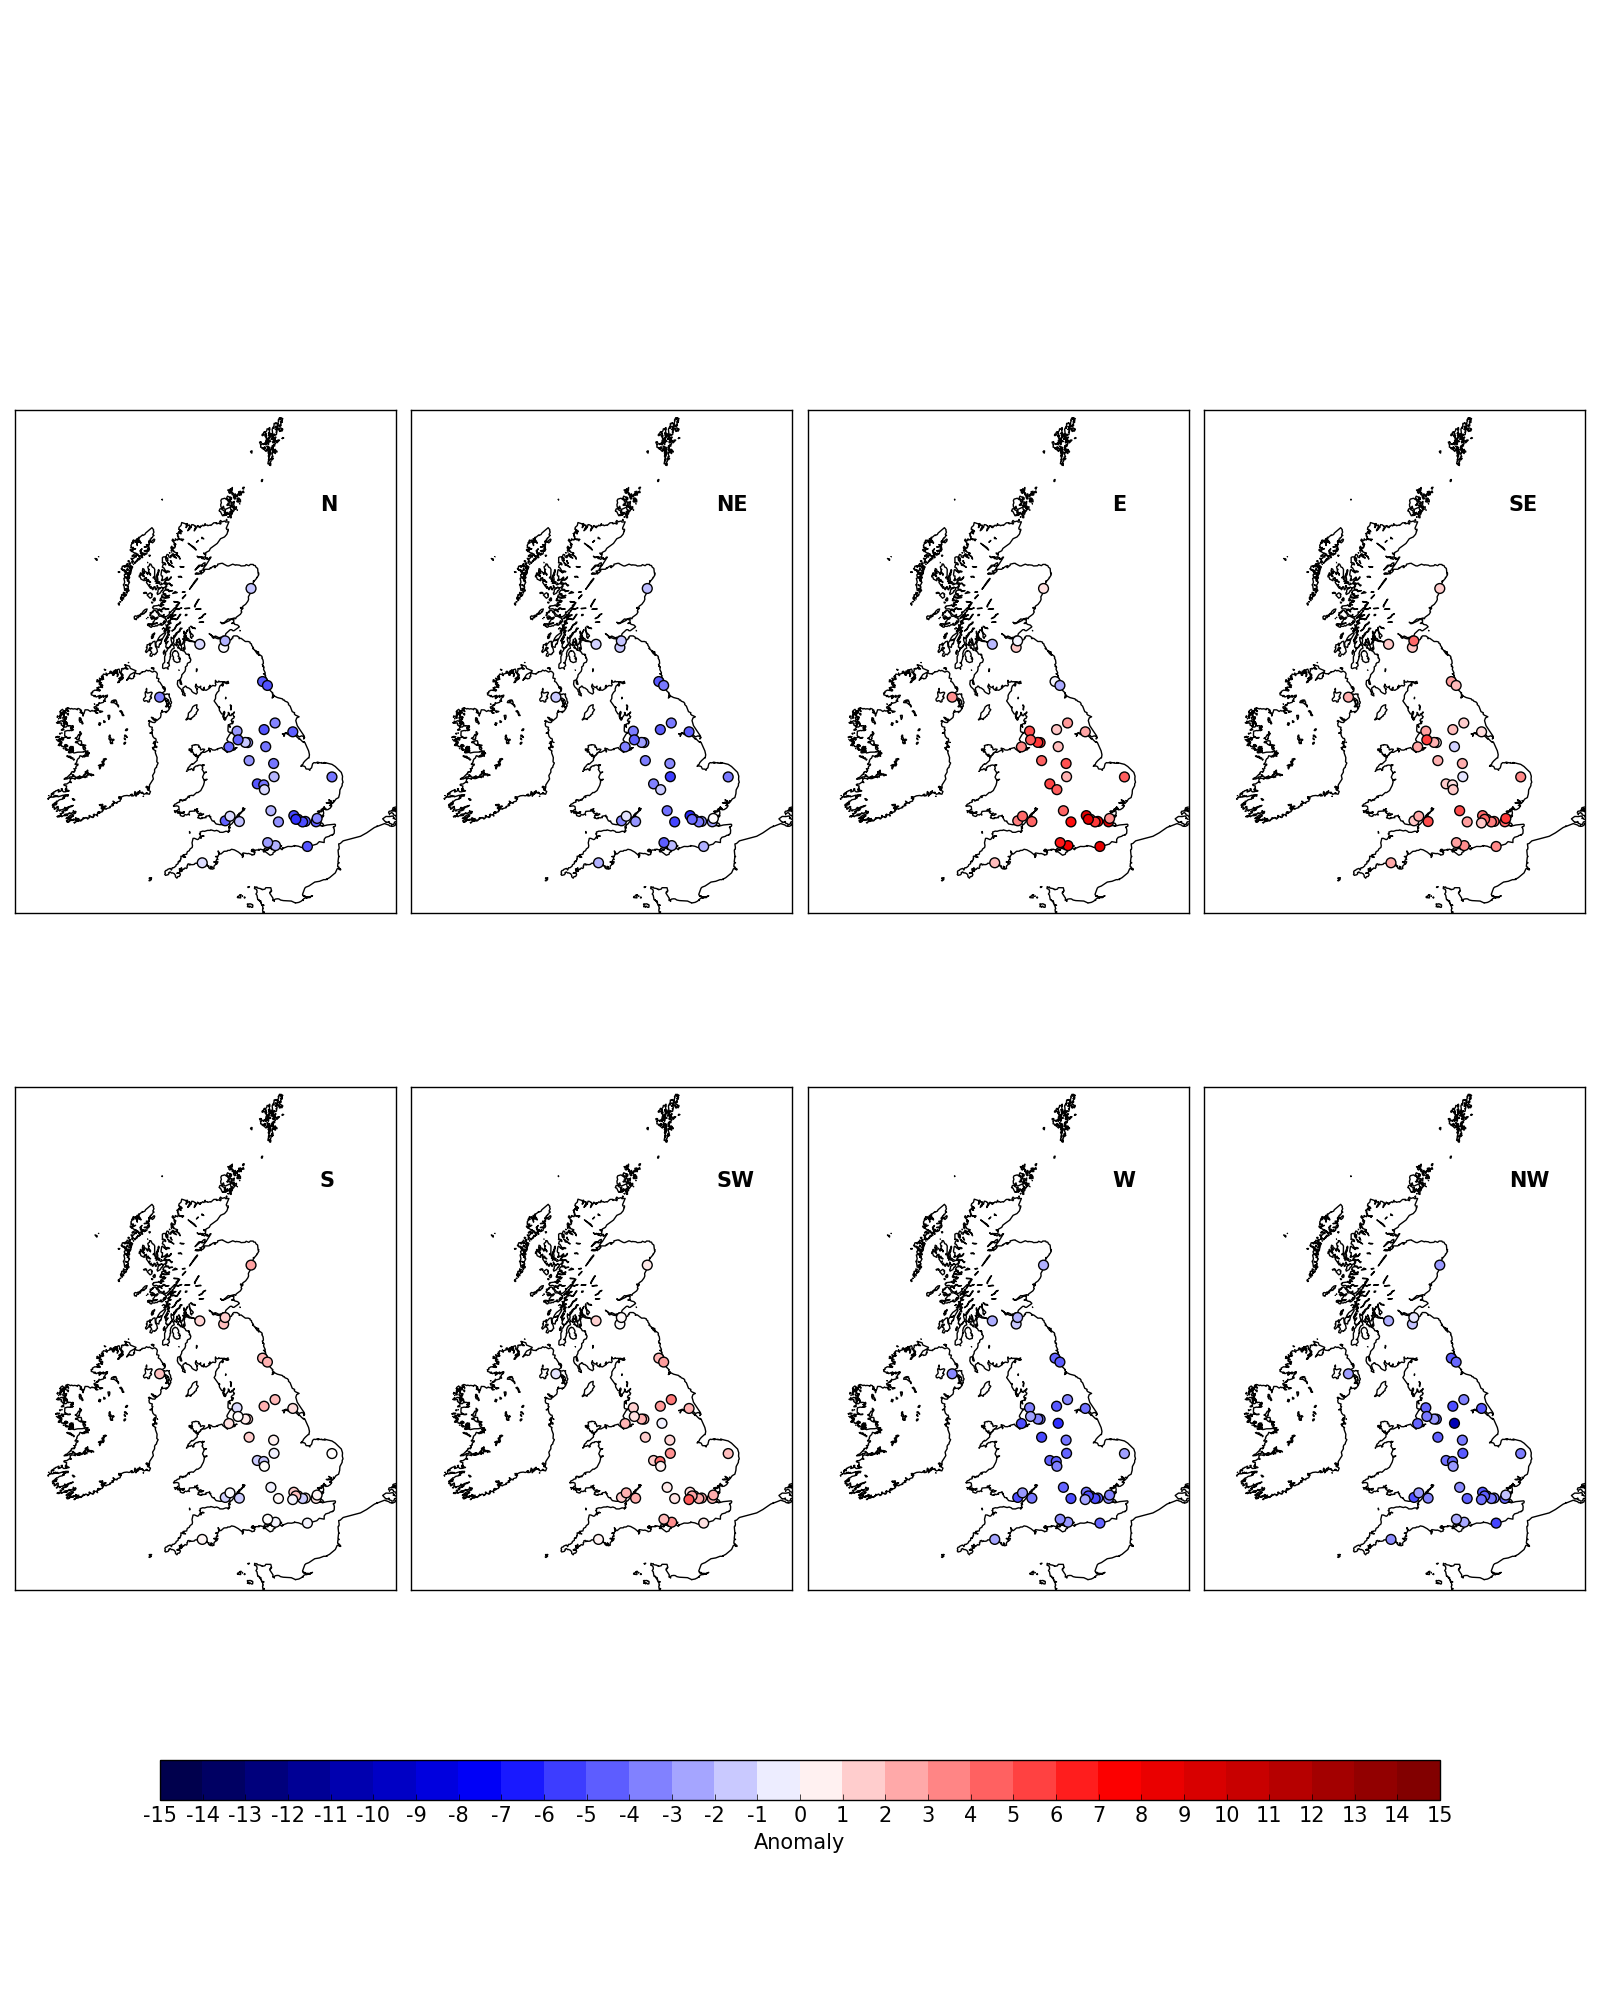
\includegraphics[height=22cm]{/nfs/see-fs-01_teaching/ee15amg/Paper_1/figures/anomalies/Autumn_90th_percentile_anomalies.png}
	\caption{Autumn 90th Anomaly}
\end{figure}

\begin{figure}
	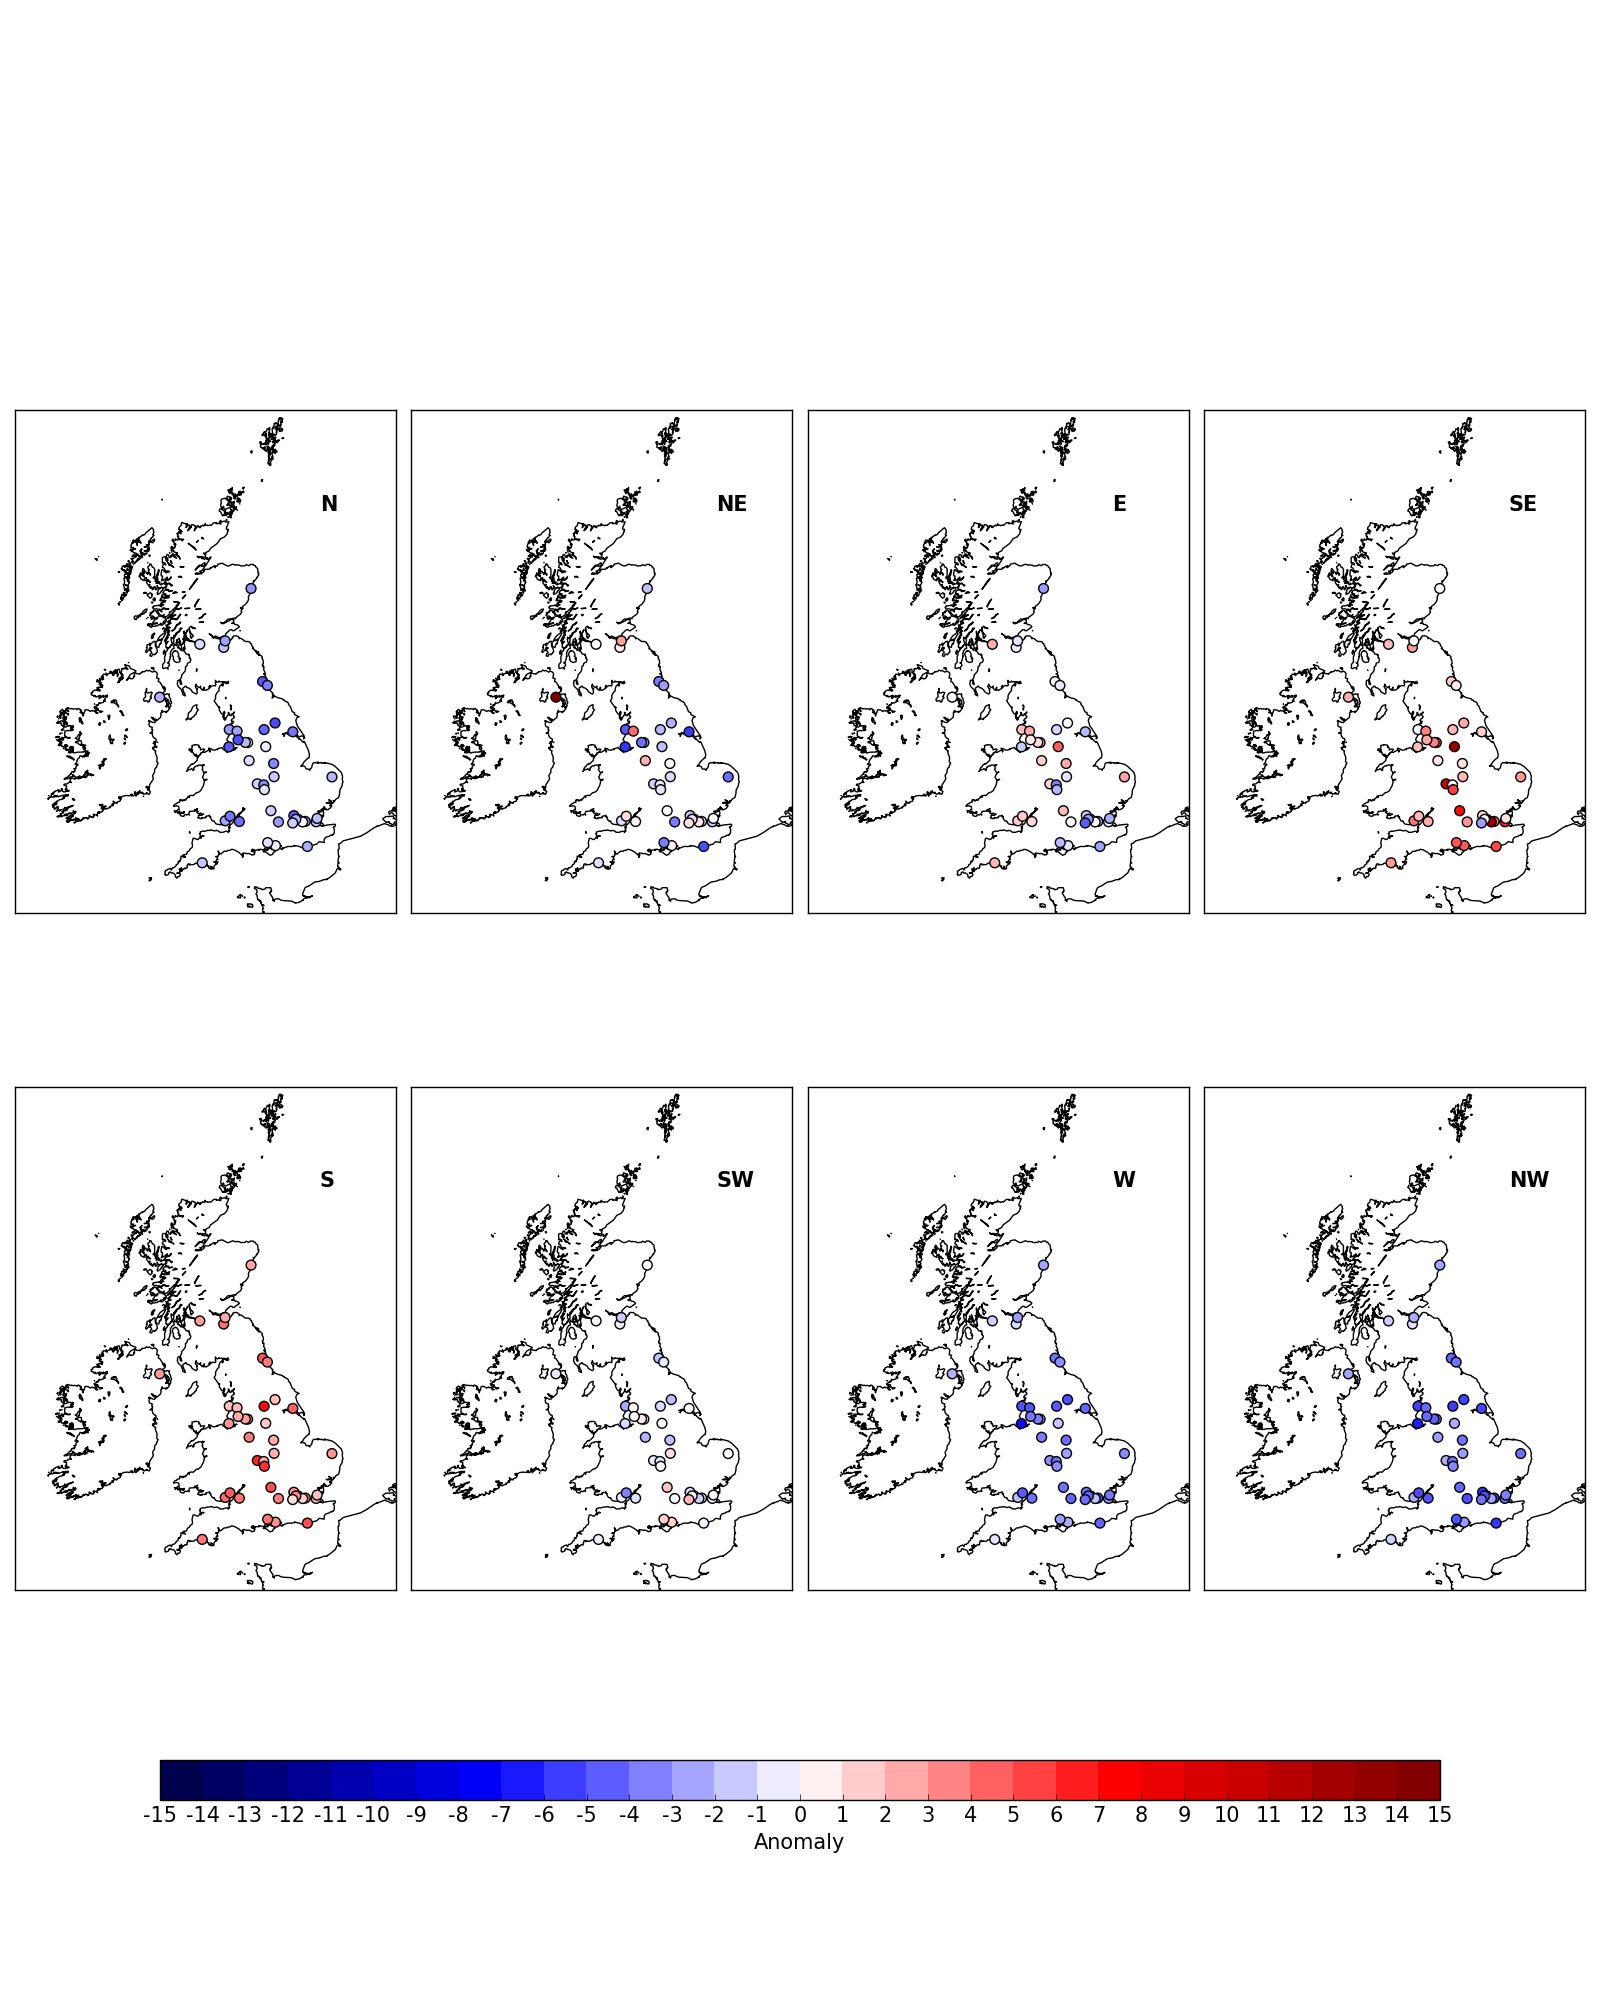
\includegraphics[height=22cm]{/nfs/see-fs-01_teaching/ee15amg/Paper_1/figures/anomalies/Winter_90th_percentile_anomalies.png}
	\caption{Winter 90th Anomaly}
\end{figure}


\textbf{Annual anomalies}

\begin{itemize}
\item  N,W,NW = most negative anomalies (more than -10)
\item NE also negative but both sites in Ireland are positive and those in Scotland are less negative than those in England. 
\item S,SE,E = most positive ( more than +10) 
\item SE positve values largest and extend furthest North 
\item E positive values as strong as SE in England but much weaker further North (+5)
\item SW is a mixed pattern but values between +3 and -3 
\end{itemize}


\textbf{Seasonal anomalies}

\begin{itemize}
\item ...............
\item \textbf{SPRING}
\item ...............
\item SE has highest anomaly values (15) but some sites have negative anomaly but no south-north or east-west divide in this. Sites that are negative anomalies as very weakly negative. 
\item S - all stations have positive anomaly but some very weak and max anomaly is less than 10.
\item E also shows positive anomaly, most strongly positive values in England with a weaker signal in Scotland and Ireland. Some negative values but most are weak apart from one in London - could be due to local pollution dominating values more than LWT and regional pollution. 
\item W and NW strongest negative anomalies - all values negative. 
\item NE and N mostly negative but some weakly positive values - less strong negative signal than W and NW.
\item ...............
\item \textbf{SUMMER}
\item ...............
\item SE pattern almost identical to Spring
\item E and S more mixed than Spring with strong positive anomalies in central England in E but weaker and sometimes negative around this. S positive signal in Scotland and N.England is weaker in Summer - tending towards zero. 
\item NW and N also weaker negative signal than spring but still negative.
\item SW almost identical to SW Spring 
\item N has a much larger proportion positive values in Summer  than Spring, with most of the negative values on the coasts - suggestive that this is local emissions dominating as oceanic air is cleaner?
\item ...............
\item \textbf{AUTUMN}
\item ..............
\item N,NE,N,NW negative anomalies (-5 to -10)
\item E highest positive anomaly (+5 - +10 for most of England), strongest in South and weaker on East coast than west coast. Scotland has weakly positive anomaly or negative anomalies at some sites.
\item SE has a sporadic signal with some sites (+5 to +10 anomaly) and other negative anomalies in central UK, also no clear north – south divide of anomalies. 
\item SW is weakly positive/weakly negative in south of UK which weakens to negative signal in Scotland 
\item S is negative/weakly positive in South of UK, in northern England to Scotland anomaly becomes more positive.
\item ...............
\item \textbf{WINTER}
\item ...............
\item Again NW, W, N all sites negative anomalies (+5 - +10)
\item NE more varied with some sites in central and western England positive anomalies and also those in central Scotland positive. 
\item E and SW very mixed signal, with some sites strongly positive and others strongly negative under SW, SW weakly positive to weakly negative and no pattern to either.
\item SE and S both strongly positive country wide with only one site in London displaying a negative anomaly in SE. SE strongest positive values in South England whereas more uniform pattern in S. 
\end{itemize}


\begin{landscape}
\begin{figure}
	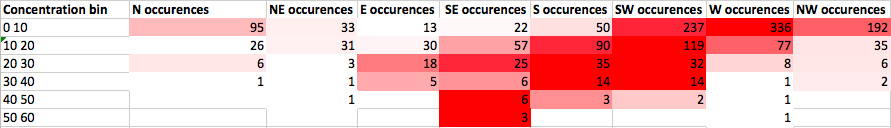
\includegraphics[height=3cm]{/nfs/see-fs-01_teaching/ee15amg/Paper_1/figures/tables/annual_conc_occurence.png}
	\caption{LWT annnual occurrences}
\end{figure}

\begin{figure}
	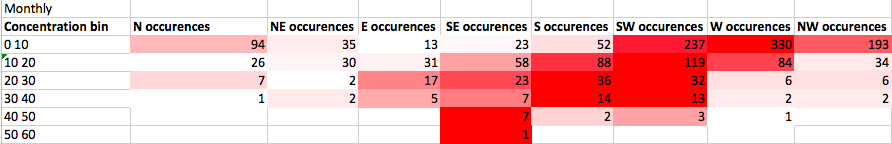
\includegraphics[height=3cm]{/nfs/see-fs-01_teaching/ee15amg/Paper_1/figures/tables/monthly_conc_occurence.png}
	\caption{LWT monthly occurrences}
\end{figure}

\pagebreak
\begin{figure}
	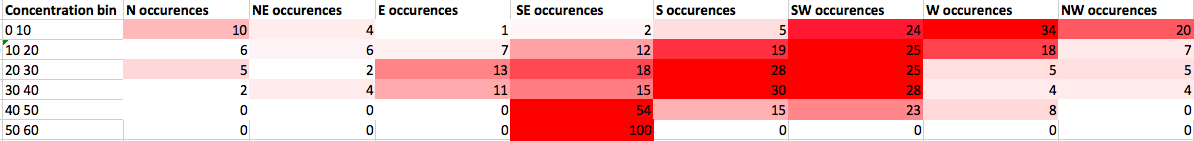
\includegraphics[height=3cm]{/nfs/see-fs-01_teaching/ee15amg/Paper_1/figures/tables/annual_conc_occurrences_percent.png}
	\caption{LWT annnual occurrences as percentage}
\end{figure}

\begin{figure}
	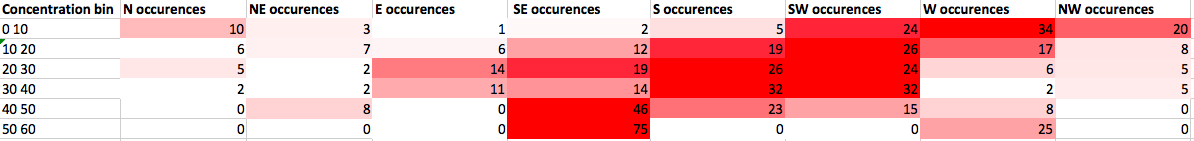
\includegraphics[height=3cm]{/nfs/see-fs-01_teaching/ee15amg/Paper_1/figures/tables/monthly_conc_occurrences_percent.png}
	\caption{LWT monthly occurrences as percentage}
\end{figure}


\begin{figure}
	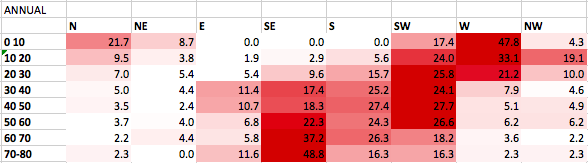
\includegraphics[height=5cm]{/nfs/see-fs-01_teaching/ee15amg/Paper_1/figures/tables/annual_lwt_conc_occ.png}
	\caption{Checked annual occurences percentages}
\end{figure}



\begin{figure}
	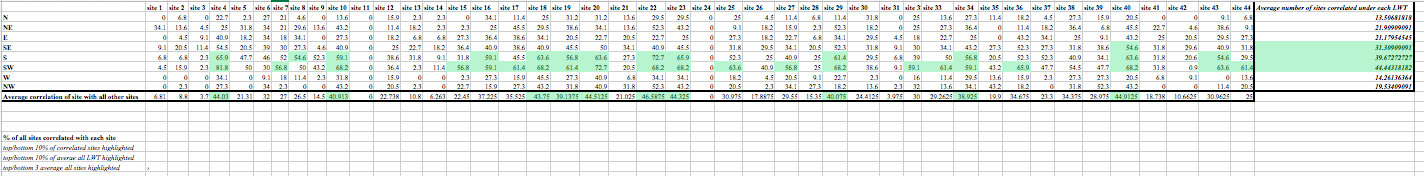
\includegraphics[height=5cm]{/nfs/see-fs-01_teaching/ee15amg/Paper_1/figures/tables/correlation_table.png}
	\caption{Correlation under LWT}
\end{figure}
\end{landscape}

\textbf{TABLES}
\begin{itemize}
\item \textbf{Monhtly occurences percentage table} each concentration bin is highlighted with darker shades to indicate higher occurrences 
\item Lowest concentrations (less than 10) occur with SW, W, NW and N flow patterns with 34\% pccurring under westerly flow. Only 1-5\% accounted for by N,E,SE and S flow patterns.
\item For concentrations between 10 and 40 this shifts from SW, SW, NW and W towards E with increasing dominance of S, SE and E and a reduction in W and NW occurrences and little change in SW (24 to 28\%). N and NE occurences also decrease from 10 and 4 to 2 and 4. 
\item At concentrations above 40 SE dominates with over half of the occurences of high concentrations observed attriutable to this flow pattern at 40-50. The other occurences at these concentrations are split between S and SW (15 and 23\%) and 8\% from westerlies. The highest concentrations observed occur under SE flow only. 
\item \textbf{Annual occurences percentage table} each concentration bin is highlighted with darker shades to indicate higher occurrences 
\item A simailar pattern is seen in the annual data, with the highest proportion of low concentration observations attributable to SW, W, NW and N flow patterns and a shift towards E,SE and S with increasing concentrations. The highest concentrations (50-50) are again dominated by SE flow (75\%) but W also accounts for 25\% of these. 

\end{itemize}
\break

\section*{Appendix}

\end{multicols}



\section*{Introduction1}

In this file, we present some tips and sample mark-up to assure your
\LaTeX\ file of the smoothest possible journey from review manuscript
to published {\it Science\/} paper.  We focus here particularly on
issues related to style files, citation, and math, tables, and
figures, as those tend to be the biggest sticking points.  Please use
the source file for this document, \texttt{scifile.tex}, as a template
for your manuscript, cutting and pasting your content into the file at
the appropriate places.

{\it Science\/}'s publication workflow relies on Microsoft Word.  To
translate \LaTeX\ files into Word, we use an intermediate MS-DOS
routine \cite{tth} that converts the \TeX\ source into HTML\@.  The
routine is generally robust, but it works best if the source document
is clean \LaTeX\ without a significant freight of local macros or
\texttt{.sty} files.  Use of the source file \texttt{scifile.tex} as a
template, and calling {\it only\/} the \texttt{.sty} and \texttt{.bst}
files specifically mentioned here, will generate a manuscript that
should be eminently reviewable, and yet will allow your paper to
proceed quickly into our production flow upon acceptance \cite{use2e}.


\section*{Formatting Citations}

Citations can be handled in one of three ways.  The most
straightforward (albeit labor-intensive) would be to hardwire your
citations into your \LaTeX\ source, as you would if you were using an
ordinary word processor.  Thus, your code might look something like
this:


\begin{quote}
\begin{verbatim}
However, this record of the solar nebula may have been partly erased by the complex history of the meteorite
parent bodies, which includes collision-induced shock,
thermal metamorphism, and aqueous alteration
({\it 1, 2, 5--7\/}).
\end{verbatim}
\end{quote}


\noindent Compiled, the last two lines of the code above, of course, would give notecalls in {\it Science\/} style:

\begin{quote}
\ldots thermal metamorphism, and aqueous alteration ({\it 1, 2, 5--7\/}).
\end{quote}

Under the same logic, the author could set up his or her reference list as a simple enumeration,

\begin{quote}
\begin{verbatim}
{\bf References and Notes}

\begin{enumerate}
\item G. Gamow, {\it The Constitution of Atomic Nuclei
and Radioactivity\/} (Oxford Univ. Press, New York, 1931).
\item W. Heisenberg and W. Pauli, {\it Zeitschr.\ f.\ 
Physik\/} {\bf 56}, 1 (1929).
\end{enumerate}
\end{verbatim}
\end{quote}

\noindent yielding

\begin{quote}
{\bf References and Notes}

\begin{enumerate}
\item G. Gamow, {\it The Constitution of Atomic Nuclei and
Radioactivity\/} (Oxford Univ. Press, New York, 1931).
\item W. Heisenberg and W. Pauli, {\it Zeitschr.\ f.\ Physik} {\bf 56},
1 (1929).
\end{enumerate}
\end{quote}

That's not a solution that's likely to appeal to everyone, however ---
especially not to users of B{\small{IB}}\TeX\ \cite{inclme}.  If you
are a B{\small{IB}}\TeX\ user, we suggest that you use the
\texttt{Science.bst} bibliography style file and the
\texttt{scicite.sty} package, both of which we are downloadable from our author help site
(http://www.sciencemag.org/about/authors/prep/TeX\_help/).  You can also
generate your reference lists by using the list environment
\texttt{\{thebibliography\}} at the end of your source document; here
again, you may find the \texttt{scicite.sty} file useful.

Whether you use B{\small{IB}}\TeX\ or \texttt{\{thebibliography\}}, be
very careful about how you set up your in-text reference calls and
notecalls.  In particular, observe the following requirements:

\begin{enumerate}
\item Please follow the style for references outlined at our author
  help site and embodied in recent issues of {\it Science}.  Each
  citation number should refer to a single reference; please do not
  concatenate several references under a single number.
\item Please cite your references and notes in text {\it only\/} using
  the standard \LaTeX\ \verb+\cite+ command, not another command
  driven by outside macros.
\item Please separate multiple citations within a single \verb+\cite+
  command using commas only; there should be {\it no space\/}
  between reference keynames.  That is, if you are citing two
  papers whose bibliography keys are \texttt{keyname1} and
  \texttt{keyname2}, the in-text cite should read
  \verb+\cite{keyname1,keyname2}+, {\it not\/}
  \verb+\cite{keyname1, keyname2}+.
\end{enumerate}

\noindent Failure to follow these guidelines could lead
to the omission of the references in an accepted paper when the source
file is translated to Word via HTML.

\section*{Handling Math, Tables, and Figures}

Following are a few things to keep in mind in coding equations,
tables, and figures for submission to {\it Science}.

\paragraph*{In-line math.}  The utility that we use for converting
from \LaTeX\ to HTML handles in-line math relatively well.  It is best
to avoid using built-up fractions in in-line equations, and going for
the more boring ``slash'' presentation whenever possible --- that is,
for \verb+$a/b$+ (which comes out as $a/b$) rather than
\verb+$\frac{a}{b}$+ (which compiles as $\frac{a}{b}$).  Likewise,
HTML isn't tooled to handle certain overaccented special characters
in-line; for $\hat{\alpha}$ (coded \verb+$\hat{\alpha}$+), for
example, the HTML translation code will return [\^{}$(\alpha)$].
Don't drive yourself crazy --- but if it's possible to avoid such
constructs, please do so.  Please do not code arrays or matrices as
in-line math; display them instead.  And please keep your coding as
\TeX-y as possible --- avoid using specialized math macro packages
like \texttt{amstex.sty}.

\paragraph*{Displayed math.} Our HTML converter sets up \TeX\
displayed equations using nested HTML tables.  That works well for an
HTML presentation, but Word chokes when it comes across a nested
table in an HTML file.  We surmount that problem by simply cutting the
displayed equations out of the HTML before it's imported into Word,
and then replacing them in the Word document using either images or
equations generated by a Word equation editor.  Strictly speaking,
this procedure doesn't bear on how you should prepare your manuscript
--- although, for reasons best consigned to a note \cite{nattex}, we'd
prefer that you use native \TeX\ commands within displayed-math
environments, rather than \LaTeX\ sub-environments.

\paragraph*{Tables.}  The HTML converter that we use seems to handle
reasonably well simple tables generated using the \LaTeX\
\texttt{\{tabular\}} environment.  For very complicated tables, you
may want to consider generating them in a word processing program and
including them as a separate file.

\paragraph*{Figures.}  Figure callouts within the text should not be
in the form of \LaTeX\ references, but should simply be typed in ---
that is, \verb+(Fig. 1)+ rather than \verb+\ref{fig1}+.  For the
figures themselves, treatment can differ depending on whether the
manuscript is an initial submission or a final revision for acceptance
and publication.  For an initial submission and review copy, you can
use the \LaTeX\ \verb+{figure}+ environment and the
\verb+\includegraphics+ command to include your PostScript figures at
the end of the compiled PostScript file.  For the final revision,
however, the \verb+{figure}+ environment should {\it not\/} be used;
instead, the figure captions themselves should be typed in as regular
text at the end of the source file (an example is included here), and
the figures should be uploaded separately according to the Art
Department's instructions.


\section*{What to Send In}

What you should send to {\it Science\/} will depend on the stage your manuscript is in:

\begin{itemize}
\item {\bf Important:} If you're sending in the initial submission of
  your manuscript (that is, the copy for evaluation and peer review),
  please send in {\it only\/} a PostScript or PDF version of the
  compiled file (including figures).  Please do not send in the \TeX\ 
  source, \texttt{.sty}, \texttt{.bbl}, or other associated files with
  your initial submission.  (For more information, please see the
  instructions at our Web submission site,
  http://www.submit2science.org/ .)
\item When the time comes for you to send in your revised final
  manuscript (i.e., after peer review), we require that you include
  all source files and generated files in your upload.  Thus, if the
  name of your main source document is \texttt{ltxfile.tex}, you
  need to include:
\begin{itemize}
\item \texttt{ltxfile.tex}.
\item \texttt{ltxfile.aux}, the auxilliary file generated by the
  compilation.
\item A PostScript file (compiled using \texttt{dvips} or some other
  driver) of the \texttt{.dvi} file generated from
  \texttt{ltxfile.tex}, or a PDF file distilled from that
  PostScript.  You do not need to include the actual \texttt{.dvi}
  file in your upload.
\item From B{\small{IB}}\TeX\ users, your bibliography (\texttt{.bib})
  file, {\it and\/} the generated file \texttt{ltxfile.bbl} created
  when you run B{\small{IB}}\TeX.
\item Any additional \texttt{.sty} and \texttt{.bst} files called by
  the source code (though, for reasons noted earlier, we {\it
    strongly\/} discourage the use of such files beyond those
  mentioned in this document).
\end{itemize}
\end{itemize}

% Your references go at the end of the main text, and before the
% figures.  For this document we've used BibTeX, the .bib file
% scibib.bib, and the .bst file Science.bst.  The package scicite.sty
% was included to format the reference numbers according to *Science*
% style.


\bibliography{nfs/see-fs-01_teaching/ee15amg/Paper_1/scibib}
\bibliographystyle{Science}



% Following is a new environment, {scilastnote}, that's defined in the
% preamble and that allows authors to add a reference at the end of the
% list that's not signaled in the text; such references are used in
% *Science* for acknowledgments of funding, help, etc.

\begin{scilastnote}
\item We've included in the template file \texttt{scifile.tex} a new
environment, \texttt{\{scilastnote\}}, that generates a numbered final
citation without a corresponding signal in the text.  This environment
can be used to generate a final numbered reference containing
acknowledgments, sources of funding, and the like, per {\it Science\/}
style.
\end{scilastnote}




% For your review copy (i.e., the file you initially send in for
% evaluation), you can use the {figure} environment and the
% \includegraphics command to stream your figures into the text, placing
% all figures at the end.  For the final, revised manuscript for
% acceptance and production, however, PostScript or other graphics
% should not be streamed into your compliled file.  Instead, set
% captions as simple paragraphs (with a \noindent tag), setting them
% off from the rest of the text with a \clearpage as shown  below, and
% submit figures as separate files according to the Art Department's
% instructions.


\clearpage

\noindent {\bf Fig. 1.} Please do not use figure environments to set
up your figures in the final (post-peer-review) draft, do not include graphics in your
source code, and do not cite figures in the text using \LaTeX\
\verb+\ref+ commands.  Instead, simply refer to the figure numbers in
the text per {\it Science\/} style, and include the list of captions at
the end of the document, coded as ordinary paragraphs as shown in the
\texttt{scifile.tex} template file.  Your actual figure files should
be submitted separately.



\end{document}




















